%% History:
%% December 2020 Veli Mäkinen removed obsolete options related to 40 cr theses
%% May 2019 Tomi Männistö, Antti-Pekka Tuovinen proofreading; 30 vs. 40 cr theses, etc.
%% May 2019 Tomi Männistö changed from babelbib to bibtex; Abstract page (and other pages as well) reformatting.
%% January–May 2019 several issues fixed by Niko Mäkitalo; long fields in abstract
%% March 2018 template file extended by Lea Kutvonen to exploit HYthesisML.cls.
%% Feb2018 This template file for the use of HYgraduML.cls was  modified by Veli Mäkinen from HY_fysiikka_LuKtemplate.tex
%% authored by Roope Halonen ja Tomi Vainio in 2017.
%% Some text is also inherited from engl_malli.tex versions by Kutvonen, Erkiö, Mäkelä, Verkamo, Kurhila, and
%% Nykänen, to accompany tktltiki.cls (by Puolakka 2002).


%% Follow comments to support use.

%%%%%%%%%%%%%%%%%%%%%%%%%%%%%%%%%%%%%%%%%%%%%%%%%%%%%%%%%
%% STEP 1: Choose options for MSc / BSc / seminar layout and your bibliographic style
%%%%%%%%%%%%%%%%%%%%%%%%%%%%%%%%%%%%%%%%%%%%%%%%%%%%%%%%%

%%  Language: 
%%      finnish, swedish, or english
%%  Pagination (use twoside by default)  
%%      oneside or twoside,
%%  Study programme / kind of report
%%      csm  = Master's thesis in Computer Science Master's Programme;
%%      tkt = Bachelor's thesis in Computer Science Bachelor's Programme;
%%      seminar = seminar report
%%  For Master's thesis choose your line or track:
%%      (30 cr thesis, 2020 onwards, Master's Programme in Computer Science = csm)
%%      software-track-2020 = Software study track
%%      algorithms-track-2020 = Algorithms study track
%%      networking-track-2020 = Networking study track
%%
%%      (30 cr thesis, Master's Programme in Computer Science = csm)
%%      sw-track-2018 = Software Systems study track
%%      alko-track-2018 = Algorithms study track
%%      nodes-track-2018 = Networking and Services study track
%%
%%      (30 cr thesis, Master's Programme in Computer Science = csm)
%%      sw-line-2017 =  Software systems subprogramme
%%      alko-line-2017 = Algorithms, Data Analytics and Machine Learning subprogramme
%%      bio-line-2017 = Algorithmic Bioinformatics subprogramme
%%      nodes-line-2017 = Networking and Services subprogramme
%%

\documentclass[english,twoside,censored,tkt,sw-line]{HYthesisML}


% In theses, open new chapters only at right page.
% For other types of documents, may ask "openany" in document.
\PassOptionsToClass{openright,twoside,a4paper}{report}
%\PassOptionsToClass{openany,twoside,a4paper}{report}

\usepackage{csquotes}
%%%%%%%%%%%%%%%%%%%%%%%%%%%%%%%%%%%%%%%%%%%%%%%%%%%%%%%%%
%% REFERENCES
%% Some notes on bibliography usage and options:
%% natbib -> you can use, e.g., \citep{} or \parencite{} for (Einstein, 1905); with APA \cite -> Einstein, 1905 without ()
%% maxcitenames=2 -> only 2 author names in text citations, if more -> et al. is used
%% maxbibnames=99 as no great need to suppress the biliography list in a thesis
%% for more information see biblatex package documentation, e.g., from https://ctan.org/pkg/biblatex 

%% Reference style: select one 
%% for APA = Harvard style = authoryear -> (Einstein, 1905) use:
\usepackage[style=authoryear,bibstyle=authoryear,backend=biber,natbib=true,maxnames=99,maxcitenames=2,giveninits=true,uniquename=init]{biblatex}
%% for numeric = Vancouver style -> [1] use:
%\usepackage[style=numeric,bibstyle=numeric,backend=biber,natbib=true,maxbibnames=99,giveninits=true,uniquename=init]{biblatex}
%% for alpahbetic -> [Ein05] use:
%\usepackage[style=alphabetic,bibstyle=alphabetic,backend=biber,natbib=true,maxbibnames=99,giveninits=true,uniquename=init]{biblatex}
%

\addbibresource{bibliography.bib}
% in case you want the final delimiter between authors & -> (Einstein & Zweistein, 1905) 
% \renewcommand{\finalnamedelim}{ \& }
% List the authors in the Bibilipgraphy as Lastname F, Familyname G,
\DeclareNameAlias{sortname}{family-given}
% remove the punctuation between author names in Bibliography 
%\renewcommand{\revsdnamepunct}{ }


%% Block of definitions for fonts and packages for picture management.
%% In some systems, the figure packages may not be happy together.
%% Choose the ones you need.

%\usepackage[utf8]{inputenc} % For UTF8 support, in some systems. Use UTF8 when saving your file.

\usepackage{lmodern}         % Font package, again in some systems.
\usepackage{textcomp}        % Package for special symbols
\usepackage[pdftex]{color, graphicx} % For pdf output and jpg/png graphics
\usepackage{epsfig}
\usepackage{subfigure}
\usepackage[pdftex, plainpages=false]{hyperref} % For hyperlinks and pdf metadata
\usepackage{fancyhdr}        % For nicer page headers
\usepackage{tikz}            % For making vector graphics (hard to learn but powerful)
%\usepackage{wrapfig}        % For nice text-wrapping figures (use at own discretion)
\usepackage{amsmath, amssymb} % For better math

\singlespacing               %line spacing options; normally use single

\fussy
%\sloppy                      % sloppy and fussy commands can be used to avoid overlong text lines
% if you want to see which lines are too long or have too little stuff, comment out the following lines
% \overfullrule=1mm
% to see more info in the detailed log about under/overfull boxes...
% \showboxbreadth=50 
% \showboxdepth=50



%%%%%%%%%%%%%%%%%%%%%%%%%%%%%%%%%%%%%%%%%%%%%%%%%%%%%%%%%
%% STEP 2:
%%%%%%%%%%%%%%%%%%%%%%%%%%%%%%%%%%%%%%%%%%%%%%%%%%%%%%%%%
%% Set up personal information for the title page and the abstract form.
%% Replace parameters with your information.
\title{Tutkielman otsikko}

% TM: Contributors to template editors now listed in the beginning of the file in comments
\author{Outi Opiskelija}
\date{\today}



% Set supervisors and examiners, use the titles according to the thesis language
% Prof. 
% Dr. or in Finnish toht. or tri or FT, TkT, Ph.D. or in Swedish... 
\supervisors{Prof.~D.U.~Mind, Dr.~O.~Why}
\examiners{Prof.~D.U.~Mind, Dr.~O.~Why}


\keywords{ulkoasu, tiivistelmä, lähdeluettelo}
\additionalinformation{\translate{\track}}

%% For seminar reports:
%%\additionalinformation{Name of the seminar}

%% Replace classification terms with the ones that match your work. ACM
%% ACM Digital library provides a taxonomy and a tool for classification
%% in computer science. Use 1-3 paths, and use right arrows between the
%% about three levels in the path; each path requires a new line.

\classification{\protect{\ \\
\  General and reference $\rightarrow$ Document types  $\rightarrow$ Surveys and overviews\  \\
\  Applied computing  $\rightarrow$ Document management and text processing  $\rightarrow$ Document management $\rightarrow$ Text editing
}}

%% if you want to quote someone special. You can comment this line out and there will be nothing on the document.
%\quoting{Bachelor's degrees make pretty good placemats if you get them laminated.}{Jeph Jacques}


%% OPTIONAL STEP: Set up properties and metadata for the pdf file that pdfLaTeX makes.
%% Your name, work title, and keywords are recommended.
\hypersetup{
    unicode=true,           % to show non-Latin characters in Acrobat’s bookmarks
    pdftoolbar=true,        % show Acrobat’s toolbar?
    pdfmenubar=true,        % show Acrobat’s menu?
    pdffitwindow=false,     % window fit to page when opened
    pdfstartview={FitH},    % fits the width of the page to the window
    pdftitle={},            % title
    pdfauthor={},           % author
    pdfsubject={},          % subject of the document
    pdfcreator={},          % creator of the document
    pdfproducer={pdfLaTeX}, % producer of the document
    pdfkeywords={something} {something else}, % list of keywords for
    pdfnewwindow=true,      % links in new window
    colorlinks=true,        % false: boxed links; true: colored links
    linkcolor=black,        % color of internal links
    citecolor=black,        % color of links to bibliography
    filecolor=magenta,      % color of file links
    urlcolor=cyan           % color of external links
}

%%-----------------------------------------------------------------------------------

\begin{document}

% Generate title page.
\maketitle


%%%%%%%%%%%%%%%%%%%%%%%%%%%%%%%%%%%%%%%%%%%%%%%%%%%%%%%%%
%% STEP 3:
%%%%%%%%%%%%%%%%%%%%%%%%%%%%%%%%%%%%%%%%%%%%%%%%%%%%%%%%%
%% Write your abstract to be positioned here.
%% You can make several abstract pages (if you want it in different languages),
%% but you should also then redefine some of the above parameters in the proper
%% language as well, in between the abstract definitions.

\begin{abstract}

Tämä dokumentti on tarkoitettu Helsingin yliopiston tietojenkäsittelytieteen osaston opin\-näyt\-teiden ja harjoitustöiden ulkoasun ohjeeksi ja mallipohjaksi. Ohje soveltuu kanditutkielmiin, ohjelmistotuotantoprojekteihin, seminaareihin ja maisterintutkielmiin. Tämän ohjeen lisäksi on seurattava niitä ohjeita, jotka opastavat valitsemaan kuhunkin osioon tieteellisesti kiinnostavaa, syvällisesti pohdittua sisältöä.


Työn aihe luokitellaan  
ACM Computing Classification System (CCS) mukaisesti, 
ks.\ \url{https://www.acm.org/about-acm/class},
käyttäen komentoa \verb+\classification{}+. 
Käytä muutamaa termipolkua (1--3), jotka alkavat juuritermistä ja joissa polun tarkentuvat luokat erotetaan toisistaan oikealle osoittavalla nuolella.

\end{abstract}

\begin{otherlanguage}{english}
\begin{abstract}
Use this otherlanguage environment to write your abstract in another language if needed.

Topics are classified according to the ACM Computing Classification System
(CCS), see 
\url{https://www.acm.org/about-acm/class}:
check command \verb+\classification{}+. A small set of paths (1--3) should be used, starting from any top nodes
referred to bu the root term CCS leading to the leaf nodes. The elements
in the path are separated by right arrow, and emphasis of each element individually can be indicated
by the use of bold face for high importance or italics for intermediate
level. The combination of individual boldface terms may give the reader
additional insight. 
\end{abstract}
\end{otherlanguage}

% Place ToC
\newpage
\mytableofcontents
\mainmatter

%%%%%%%%%%%%%%%%%%%%%%%%%%%%%%%%%%%%%%%%%%%%%%%%%%%%%%%%%
%% STEP 4: Write the thesis.
%%%%%%%%%%%%%%%%%%%%%%%%%%%%%%%%%%%%%%%%%%%%%%%%%%%%%%%%%
%% Your actual text starts here. You shouldn't mess with the code above the line except
%% to change the parameters. Removing the abstract and ToC commands will mess up stuff.
%%
%% You may wish to include material to avoid browsing the definitions
%% above. Command \include{file} includes the file of name file.tex.
%% As a side effect, subsequent inclusions may force a page break.

% BSc instructions
%\chapter{Johdanto}


Kaikessa julkaistavaksi tarkoitetussa tekstissä kirjoittajan luomisen ja
esitystavan vapautta rajoittavat monet ohjeet ja tarkatkin määräykset.

Parhaimmillaan lukijalle ja kirjoittajalle yhteinen, tuttu säännöstö luo
eräänlaisen tukiverkoston, joka tukee sanoman siirtymistä vääristymättä.
Kirjoituksen lukija löytää kirjoituksesta helpommin olennaisen sisällön,
jos kirjoituksen ulkoasu ja sisällön rakenne vastaavat hänen
tottumuksiaan. Sama koskee myös kirjoittajaa. Noudattaessaan valmista
esitystapamallia kirjoittajan ei tarvitse käyttää aikaansa itse työn
kannalta toissijaisten seikkojen miettimiseen, vaan hän voi keskittyä
hiomaan tekstin sisältöä. Siksi kannattaa harjoitella myös työn ulkoasua
koskevien ohjeiden noudattamista, vaikka omasta mielestään osaisikin
valita esitykselleen ohjetta paremman muodon.

Tämä kirjoitus on tarkoitettu Helsingin yliopiston
Tietojenkäsittelytieteen osastoon alempien opinnäytteiden ja
harjoitusten ulkoasun ja rakenteen ohjeeksi. Ohje soveltuu siten
kandidaatintutkielman kirjoittamisen kurssille, ohjelmistotuotantoprojekteihin, seminaareihin ja
pro gradu -tutkielmiin. (Kirjoitus on päivitetty uusintapainos aiemmista
ohjeista, jotka kurssin luennoijat ovat laatineet \citep{erkio01,erkiomakela96,erkio94,verkamo92}.)

Tyylimäärittely on saatavissa pdflatex- ja word-versiona.
Tyylimäärittelyitä valitessa on huomattava ohjeet tekstien syöttöön
liittyvässtä koodauksesta (UTF8,ISO 8859-15).
Tämän kirjoituksen tukena sopivat käytettäväksi tavanomaiset latex- tai
word-oppaat. 

\chapter{Kirjoituksen rakenne}

Tarkastellaan aluksi tieteelliseltä tekstiltä odotettuja
kirjoituksen osia. Samoihin asioihin on luonnollisesti syytä
kiinnittää huomiota myös muussa teknisessä kirjoittamisessa. Huomattakoon, että tämä teksti ei ole tieteellinen teksti, eikä siten itse sisällä kaikkia niitä elementtejä, jotka tieteellisen tekstin sisällölliseen antiin kuuluvat. Tällaisia puutteita ovat esimerkiksi johdannon tutkimuskysymyksen asettelun puuttuminen sekä arvoivan materiaalin puute tekstin lopussa, sekä yhteenvedon latteus.
Teksti rajoittuu siten otsikkonsa mukaisesti vain tekniseen sisällön asetteluun.

\section{Tiivistelmä}



Tiivistelmäsivu sisältää seuraavat osat: työn bibliografiset tiedot,
tiivistelmäteksti, aiheluokat ja avainsanat. Bibliografiset tiedot
koostuvat työn otsikosta, tekijän nimestä, julkaisupaikan tiedoista,
julkaisuajankohdasta ja sivumäärästä.

Tiivistelmäteksti on lyhyt, yleensä yhden kappaleen mittainen
(maksimissaan noin 100 sanaa) selvitys
kirjoituksen tärkeimmästä sisällöstä: mitä on tutkittu, miten on
tutkittu ja mitä tuloksia on saatu.


Aiheluokat kuvataan ACM Computing Classification System -luokituksen (CCS)
luokituksen mukaisesti. Luokittelussa käytetään täysia polkuja juurisolmun CCS osoittamista lähtöposteistä lehtisolmuihin. Polkuja voi antaa 1-3 aihepiirien soveltuvuuden mukaan, mitä alempi opinnäyte, sen vähemmän polkuja se tarvitsee. 
Poluissa tasot erotetaan toisistaan nuolella eteenpäin. Kun  polun nimisanoja arvioidaan suhteessa työn sisältöön, merkitään boldface-fontilla tärkein termi, italics-fontilla toiseksi tärkein. Näin menetellään, mikäli jotkin termeistä ovat olennaisesti paremmin kuvaavia kuin muut polun termit. Nimettyjen polkujen lisäksi lukija voi siten tarkastella lisäulottuvuutena myös tärkeiksi merkittyjen termien joukkoa sinänsä.
Avainsanoiksi valitaan kirjoituksen sisältöä
keskeisesti kuvaavia käsitteitä.

\section{Johdanto}


Johdannon tarkoituksena on kertoa yleiskielisesti
työn tavoite. Kerrotaan (kuten tiivistelmässäkin, mutta laveammin),
mitä on tutkittu, miten on tutkittu ja mitä tuloksia on saatu.
Jotta kysymyksenasettelu ja tulokset on lukijan helppo oikein tulkita on syytä aloittaa johdanto asettelemalla tutkimus asiayhteyteensä, esimerkiksi kertomalla aluksi, minkälaisessa yhteydessä tarkasteluun otettavat haasteet esiintyvät ja keiden on ratkaisuista tarkoitus hyötyä.

Johdannon pituus määräytyy suhteessa koko kirjoitelman pituuteen.
Parisivuinen kirjoitus ei erikseen otsikoitua johdantoa kaipaa, sillä
se itsessään on laajennettu tiivistelmä. Kymmensivuisen
kirjoituksen johdanto voi olla vaikkapa sivun tai puolentoista
mittainen. Pro gradu -tutkielman 50-70-sivuiseen kokonaisuuteen
tuntuu 2-4-sivuinen johdanto kohtuulliselta. 

Johdanto kertoo siis lyhyessä, yleistajuisessa muodossa
koko kirjoitelman kysymyksenasettelun, juonen sekä tulokset ja johtopäätelmät.
Tämän luettuaan lukija voi päätellä, haluaako syventyä asiaan tarkemmin
lukemalla koko kirjoituksen.


\section{Käsittelyluvut}

Käsittelylukujen työnjako määräytyy käsiteltävän asian luonteen
mukaisesti.
Lukijan ohjailemiseksi kukin pääluku kannattaa aloittaa lyhyellä
kappaleella, joka paljastaa mikä kyseisen luvun keskeisin sisältö on ja
kuinka aliluvuissa asiaa kehitellään eteenpäin.
Erityisesti kannattaa kiinnittää huomiota siihen, että lukijalle ilmaistaan selkeästi miksi kutakin asiaa käsitellään ja miten käsiteltävät asiat suhtautuvat toisiinsa. 

Jäsentelyongelmista kielivät tilanteet, joissa
alilukuja on vain yksi, tai joissa käytetään useampaa kuin
kahta tasoa (pääluku ja sen aliluvut). Kolmitasoisia
otsikointeja saatetaan tarvita joissakin teknisissä
dokumenteissa perustellusti, mutta nämä muodostavat poikkeuksen.

Perusohjeena on käyttää tekstin rakenteellisesti painokkaita paikkoja,
kuten lukujen avauksia ja teksikappaleiden aloitusvirkkeitä
juonenkuljetukseen ja informaatioaskeleiden sitomiseen toisiinsa.
Tekstikappaleiden keskiosat, samoin kuin lukujen keskiosat selostavat
asiaa vähemmän tuntevalle yksityiskohtia, kun taas aihepiirissä jo
sisällä olevat lukijat voivat alkuvirkkeitä silmäilemällä edetä
tekstissä tehokkaasti eksymättä tarinan juonesta.

Kullakin kirjoittajalla on oma temponsa, joka välittyy lukijalle
tekstikappaleiden pituudessa ja niihin sisällytettyjen ajatuskulkujen
mutkikkuudessa. Kussakin tekstikappaleessa pitäisi pitäytyä vain yhdessä
informaatioaskelessa tai olennaisessa päättelyaskelessa, muuten juonen
seuraaminen käy raskaaksi olennaisten lauseiden etsiskelyksi. Yksivirkkeisiä
tekstikappaleita on syytä varoa. 



\section{Lähdeviittausten käyttö}


Olennaisia opittavia asioita viittaustekniikoissa ovat viitteen paikka
tekstissä, oikea lähdeluettelojärjestys valitun viitetyylin parina sekä
taito ja tahto noudattaa annettua tyylimääräystä. Väitöskirjoissa ja
lehti- tai konferenssiartikkeleissa tekstin hyväksyminen riippuu myös
näiden yksityiskohtien asianmukaisesta käsittelystä. Tästä syystä
laitoksella nähdään tarpeelliseksi opiskelijoiden tutustua edes
pinnallisesti myös muihin tyylilajeihin ja oppia käyttämään
automatisoituja muotoilutyökaluja tehokkaasti, jolloin tyylimuutokset
ovat tehokkaita.

Lähdeviitteet sijoitetaan aina virkkeen sisäpuolelle. Siten esimerkiksi
tekstikappaleen lopussa irrallaan oleva viite ei ole asiallinen. Tilanne
ei muutu, vaikka viite sujautettaisiin tekstikappaleen viimeisen
virkkeen sisään. 
Lähdeviittauksen yhteyteen merkitään mukaan tarkentavat
sivunumerot, mikäli lukijan olisi työlästä löytää asianomainen kohta
viitatusta lähteestä. 


Tehokkaita viitteensijoittelupaikkoja ovat esimerkiksi uuden käsitteen
nimeämiskohta ja virkkeen loppu kun kyseessä on lähteestä lainattu
väite. On myös muistettava lainausmerkkien käyttö silloin kun tehdään
suoria lainauksia.

Tekstin jäsentelyn on tuotava selkeästi esiin, mihin asiaan viite
liittyy. Samalla tulee ymmärrettäväksi se, kuinka pitkään
tekstikatkelmaan ko. viite liitetään. Ei ole siten asiallista aloittaa
lukua nimeämällä yhtä tai useampaa lähdettä luvun taustaksi, vaan
viitteitä on kiinnitettävä täsmällisemmin väitteisiin ja käsitteisiin.
Luvun avaus viitetiedolla voi olla oire myös suuremmasta ongelmasta:
lähderiippuvuudesta. Aloitteleva kirjoittaja helposti toistaa lähteestä
oppimaansa ilman että tarpeellinen analysointi ja prosessointi suhteessa
muuhun opittuun olisi vielä tapahtut.

Viitteillä ja sanamuodolilla on
myös tuotava selkeästi esiin se, mikä teksissä on lainattua ja mikä oman
pohdinnan ja valikoinnin tulosta.


Lähdeviittauksiin käytetään Tietojenkäsittelytieteen osastolla
numeroitua tyyliä ja APA-tyyliä, valinnan näiden välillä tekevät kunkin
ryhmän valvoja ja ohjaaja yhdessä. 
Numeroitu tyyli on esimerkiksi IEEE- ja
ACM-julkaisuissa yleisesti käytetty ja puolustaa siten paikkaansa.
APA-tyyli on poikkeuksellinen ns. kovissa tieteissä, mutta monet
valvojista pitävät siitä sen luettavuuden vuoksi. Numeroita joutuu nimiä
useammin tarkistamaan lähdeluettelosta, sillä tarkastus- ja
arvointiprosessiin kuuluu arvioida myös lähteiden valitaa ja niiden
käyttötapaa.





\section{Yhteenveto}

Yhteenveto  vaatimattomimmillaan on vain lyhyt kertaus kirjoituksen
keskeisistä asioista. Arvokkaamman yhteenvedon saa aikaan kommentoimalla
 työn tulosten arvoa, työn liittymistä ympäristöön ja
tulevaisuudennäkymiä. Tällaiset arviot  huolellisesti
perusteltava.

\section{Lähdeluettelon laatiminen}

Tieteellisen kirjoittamisen kurssin töiden lähdeluetteloiden
laatimisessa noudatetaan seuraavia ohjeita.

Niiden taustalla on kaksi
keskeistä pyrkimystä: tehdä viitatun lähteen hankkiminen luettavaksi
mahdollisimman helpoksi ja ilmaista, millaisen arviointiprosessin
läpi käyneeseen kirjoitukseen vedotaan.
Näistä syistä
\begin{itemize}
\item lähdeviitteen tulee aina olla niin tarkka, että
lähde on sen perusteella tunnistettavissa ja löydettävissä luetteloista
ja kirjastoista,
\item erityyppisten lähteiden (kirjat, konferenssit, lehdet) on erotuttava
toisistaan
ja
\item luettelon eri osien tulee olla mahdollisimman
yhdenmukaisia, erityisesti lähdetyypin sisällä.
\end{itemize}


Riippumatta käytettävästä viitetyylistä, 
lähteet ovat Tietojenkäsittelytieteen osaston opinnäytteiden lähdeluetteloissa tekijän nimen mukaisessa aakkosjärjestyksessä,
saman tekijän (tekijäryhmän) työt julkaisuajan mukaisessa
järjestyksessä. Jos jollakin lähteellä ei ole henkilötekijää, se
aakkostetaan julkaisun nimen mukaisesti. 

Kustakin lähteestä annetaan seuraavat tiedot, edelleen viitetyylistä riippumatta:
\begin{itemize}
\item (tarvittaessa lähdeviitelyhenne).
\item
tekijän tai tekijöiden nimet (sukunimi, etunimien alkukirjaimet)
alkuperäisessä järjestyksessään; jos tekijöitä on enemmän kuin kolme,
voidaan toimia siten, että
vain ensimmäinen tekijä nimetään ja muiden tilalle kirjoitetaan {\em et
al.}
\item
julkaisun tai artikkelin nimi alkuperäisessä muodossaan
\item
julkaisupaikan tiedot:
\begin{itemize}
\item
kirjasta: kustantaja, julkaisupaikka (voidaan jättää pois, jos kyseessä
on tunnettu kustantaja), vuosi ja
\item
lehtiartikkelista: lehden nimi, volyymi, numero, vuosiluku ja kuukausi (suluissa),

\item
artikkelikokoelmassa (esim. konferenssijulkaisussa) ilmestyneestä
artikkelista:
\begin{itemize}
\item kokoelman nimi, toimittaja, kustantaja, julkaisupaikka ja vuosi
{\em tai}
\item konferenssin nimi, järjestäjä, paikka ja aika,
\end{itemize}
\item
raportista: julkaisusarja, raportin numero, julkaisupaikka, julkaisija ja vuosi
ja
\item
www-lähteestä: verkko-osoite, voimassaoloajankohta, mahdollisesti
viittausajankohta hakasuluissa
\end{itemize}
\item
sivunumerot, mikäli lähteenä käytetty julkaisu on artikkeli tai kokoomateoksen itsenäinen luku.
\end{itemize}

Normaaliin suomalaiseen tapaan artikkelin nimessä ainoastaan
ensimmäinen sana kirjoitetaan isolla alkukirjaimella, sen sijaan
konferenssien ja kokoelmajulkaisujen nimissä käytetään isoa
alkukirjainta jokaisen sanan alussa (artikkelisanoja ja prepositioita
lukuunottamatta). Katso mallia oheisista esimerkeistä.
Kokoelman nimen edessä on syytä selvyyden vuoksi käyttää sanaa {\em
Teoksessa}, paitsi kun on kysymys konferenssijulkaisusta, jonka nimi
alkaa lyhenteellä {\em Proc.} (sanasta Proceedings). Tällöin ei tarvita
mitään täydennystä.
Tämän eron näkee esimerkiksi vertaamalla
lähdeviitteiden~''\citep{dantowsley90}''
ja~''\citep{gannonetal89}'' ulkoasuja.

WWW-lähteiden käytössä on syytä muistaa, että verkossa julkaisukynnys on
olematon. Kannattaa siten keskittyä tunnettujen tieteellisten
kustantajien julkaisuihin ja niihin teknisiin standardeihin, joille WWW
on ainoa julkaisukanava. Mikäli sama julkaisu on saatavissa myös
perinteisessä muodossa, viitataan ensisijaisesti siihen ja käytetään
verkko-osoitetta lisätietona. Lähdeluettelossa on annettu esimerkit
useita kanavia julkaistusta kirjoituksesta~\citep{abiteboul,dietinger} sekä pelkästään
WWW-julkaisuna
leviävästä standardista~\citep{bray}.

Erityisesti varoitetaan Wikipedian käytöstä tieteellisessä tekstissä.
Vaikka sen avulla on helppo alustavasti tutustua joihin aihepiireihin ja
asiantuteva lukija voisi teksin kelvolliseksi tiettynä hetkenä
hyväksyäkin, ei se foorumina millään lailla täytä tieteellisesti
vertaisarvoidun tutkimusfoorumin kriteerejä.
Jos Wikipedia-artikkelia  ei mitenkään malta ajankuvana olla mainitsematta, käytettäköön jotain muuta kuin lähdeviitetekniikkaa tähän taiteelliseen otteeseen, vaikkapa alaviitteitä. Olennaista silloinkin on, että tieteellinen sisältö ei tule tällä korvatuksi vaan sen puute korostetuksi.

WWW-lähteeseen viittaamisessa pätevät samat periaatteet kuin
perinteisiin lähteisiin viitattaessa: lähdeviitteessä ilmaistaan
otsakkeet, kirjoittajat, toimittajat js muut seikat. Eroa on ainoastaan
verkko-osoitteen ja sen voimassaoloajankohdan ilmaisemisessa. Mikäli
lähde on julkaistu ainoastaan verkossa, voidaan web-osoitetta (URL)
käyttää vastaavasti kuin perinteisen julkaisun paikannusinformaatiota
(lehden ja se numeron julkaisutiedot). Lähdeluettelossa on WWW-viittausten yhteydessä aina syytä ilmaista päivämäärä, jolloin linkin voimassaolo ja lähteen sisältö on tarkastettu.
Esimerkkeinä verkkoviitteistä soveltuvat seuraavat:
\begin{itemize}
\item Gergen, Kenneth (1999) Narrative, Moral Identity and Historical
Consciousness: a Social Constructionist Account.
http://www.swarthmore.edu/SocSci/kgergen1/text3.html. Haettu 11.6.1999.
\item 	
Ritala-Koskinen, Aino and Valokivi, Heli (2006) The Role of Development
Skills in Social Work Practice Education in Finland. Social Work and
Society, The International Online-Only Journal 4(2006)1.
http://www.socwork.net/2006/1/series/transition/ritalakoskinenvalokivi.
Viitattu 30.8.2006.
\item Heinisuo, Rami and Ekholm, Kai (1997) Elektronisen viittaamisen
opas. Jyväskylän yliopiston kirjaston julkaisuja n:o 40. Jyväskylä:
Jyväskylän yliopiston kirjasto. http://www.pori.tut.fi/~multisil/evo/.
Viitattu 29.8.2006.
\end{itemize}

Kirjoituksen lähdeluettelossa luetellaan täsmälleen ne lähteet, joihin
viitataan kirjoituksen tekstiosassa. Tämän kirjoituksen lähdeluettelo on
tarkoitettu lähinnä esitystavan esimerkiksi, mistä syystä siinä on
''ylimääräisiä'' lähteitä.


Pääsääntöisesti julkaisun tai artikkelin nimen perään tulee piste,
samoin kunkin lähteen bibliografisten tietojen perään. Muut tiedot
erotetaan toisistaan pilkulla. Useimmissa tapauksissa  
voidaan noudattaa teknisten välineiden antamaa mallia, sillä edellytyksellä, että ylläolevat vaatimukset muuten täyttyvät.



\chapter{Ulkoasulliset seikat}

  Tässä luvussa käsitellään yleisimpiä
tekstin tekniseen esittämiseen liittyviä seikkoja.  

\section{Työn osien järjestys}

   Kirjoituksen alussa on aina
erillinen, mallin mukainen kansilehti. Toisena sivuna on
tiivistelmäsivu, sen jälkeen sisällysluettelo (yksi tai useampia
sivuja) ja sitten varsinainen teksti. Sivunumerointi aloitetaan vasta
ensimmäiseltä tekstisivulta (arabialaisella ykkösellä). (Tarkat
jättävät ykkössivun numeromerkittä.) Sisällysluetteloon merkitään
kaikki (numeroidut) otsikot ja vastaavat sivunumerot. Monet
tekstin\-käsittelyjärjestelmät muodostavat itse sisällysluettelon,
jolloin kirjoittajan ei tarvitse huolehtia luettelon sivunumeroiden
päivittämisestä tekstin kehittyessä. Sisällysluettelo\-sivu ja sitä
edeltävät sivut voidaan haluttaessa numeroida erikseen (roomalaisin
numeroin) esimerkiksi tämän mallin mukaisesti.  

Varsinaisen tekstin
jäljessä, mutta itse työhön kuuluvana on ensimmäisenä lähdeluettelo,
jonka otsikkoa ei numeroida. Lähdeluettelon jälkeen sijoitetaan
mahdolliset liitteet, jotka otsikoidaan ja varustetaan sisäisillä
sivunumeroilla.  



Mikäli kuvista, algoritmeista
ja taulukoista halutaan tehdä yhtenäinen luettelo, sijoitetaan
luettelot sisällysluettelon jälkeen. Luetteloiden käyttöarvosta on
eriäviä mielipiteitä, joten niiden laatimiseen ei varsinkaan ilman
tekstinkäsittelyjärjestelmän tukea kannata ryhtyä ilman tarkastajan
erityistä toivetta.  

Mikäli kirjoitukseen erityissyistä halutaan
liittää aakkosellinen hakemisto, sijoitetaan se lähdeluettelon jälkeen
ennen liitteitä. Indeksi merkitään sisällysluetteloon samoin kuin
lähdeluettelo (numeroimaton luku). Mikäli indeksin tekemiseen
ryhdytään, on syytä käyttää tekstinkäsittelyjärjestelmän tarjoamaa
automatiikkaa.

Teksin luonnollisen juonenkuljetuksen mukana esiin
tulevien käsitteiden määrittelyjen sijasta ei pidä yrittää sen enempää
pakata kaikkia määritelmiä johdantoon kuin laatia johdantoa ennen
käsitelistaa tai lyhenteiden selityslistaa. Kumpikaan ei sovi
tavanomaiseen argumentoivaan tieteelliseen tekstityyliin, vaikka
teknisessä yhteydessä niillä liitteinä voi olla lisäarvoa.


\section{Tekstin yleinen sijoittelu}

Lopullinen tutkielmaversio voi olla yksi- tai kaksipuoleiseksi aseteltua
ja riviväliltään 1,5 tai 1.  Erityyppisissä
teksteissä haasteet ja asetteluvaatimukset voivat olla erilaiset. Erota
kappaleet toisistaan yhdellä tyhjällä rivillä tai
käytä tekstinkäsittelytyökalujen ominaisuuksia
hyödyksesi ja määrittele tekstikappaleiden väliin jäävä tila hieman
normaalia riviväliä suuremmaksi.

Kirjoituksen lukujen, kuvien ja taulukoiden erottumisen kannalta
tärkein keino on riittävän tilan käyttö niiden ympärillä. Kuvan ja
nimekkeen tulee olla selkeästi yksi kokonaisuus, joka eroaa muusta
tyhjän tilan rajaamana. Kuvan tai taulukon on aina numerointinsa ja
nimekkeensä kanssa mahduttava yhdelle sivulle tai varmasti
kaksipuolisena paperidokumenttina tarkasteltavassa tekstissä aukeamalle.
Kuvissa fonttikoko ei saa alittaa 8 pistettä.



Jos uusi luku tulisi alkamaan aivan sivun alareunasta (vain yksi tai
kaksi riviä varsinaista tekstiä), aloita mieluummin uusi sivu. Jokaista
uutta lukua ei kuitenkaan ole tarpeen --- etenkään lyhyessä
kirjoituksessa --- aloittaa uudelta sivulta: jos kirjoituksessa on
paljon melkein tyhjiä sivuja, lukija voi epäillä, että kirjoittaja on
yrittänyt saada kirjoituksensa näyttämään pitemmältä kuin se onkaan. 
 Tyhjää tilaa kannattaa käyttää hyödyksi myös kuvien ja taulukoiden
yhteydessä. Erityisesti jos kirjoituksessa käytetään kauttaaltaan samaa
tekstityyppiä, tyhjät rivit ovat välttämättömiä erottamaan esimerkiksi
tekstiä ja taulukkoa toisistaan. Tyhjä tila on halpaa, mutta se lisää
selkeyttä ja luettavuutta.  


\section{Kuvat ja taulukot}


Kuva tai taulukko sijoitetaan mahdollisimman lähelle
(ensimmäistä) tekstikohtaa, jossa siihen viitataan, ei kuitenkaan
kyseistä viittausta aikaisemmaksi.
Tekstissä on syytä myös kertoa, mitä kuvalla halutaan havainnollistaa.
Kuvan voi lukea monella eri tavalla, joten lukijaa on ohjattava.

Kuvaa ei pidä sijoittaa välittömästi luvun otsikon alle, vaan on
aloitettava tekstillä. Kuvaa ei pidä sijoittaa keskelle tekstikappaletta
(saati virkettä), paitsi jos kuva tulee sivun alkuun tai loppuun eikä
kappaleen jatkumisesta tule epäselvyyttä.

Kuvan ei aina tarvitse olla välittömästi viittaavan kappaleen
perässä. Esimerkiksi viittauskohdan ja
vasta seuraavalle sivulle mahtuvan kuvan väliin jäävää sivun loppuosaa
ei jätetä tyhjäksi. Kuvaa ei kuitenkaan pidä viedä seuraavaa
sivua kauemmas viittauskohdasta.


Varsinaista kuvan esittämistä havainnollistaa kuva~\ref{kuvaesimerkki}.
Huomiota on kiinnitettävä kuvan osien ja tekstimerkintöjen näkyvyyteen,
kuvan numerointiin ja otsikointiin. 

\begin{figure}[ht]
%\begin{figure}[tbh] t= top, b = bottom, h=here
\ \newline
\begin{center}
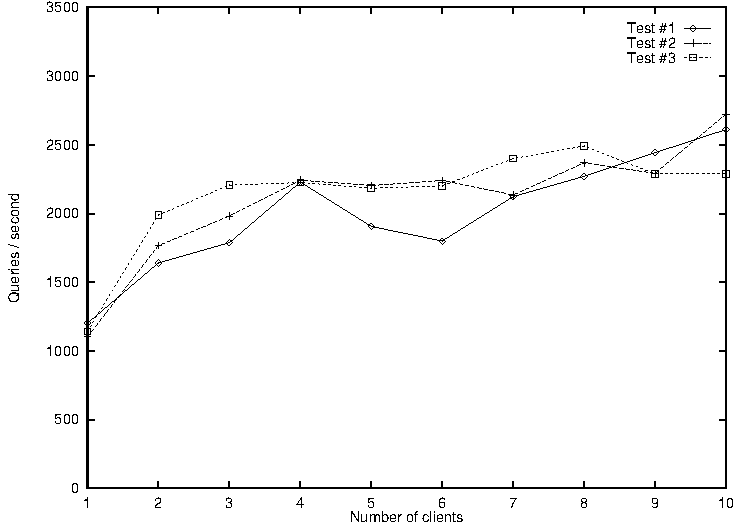
\includegraphics[width=0.75\textwidth]{kuvaesimerkki.pdf}
\caption{Kuvan elementit.}
\label{kuvaesimerkki}
\end{center}
\end{figure}


Kuvien kokoon on kiinnitettävä huomiota. Käytettyjen merkintöjen
on oltava helposti luettavissa ja selkeät. Esimerkiksi
suorituskykykäyriä esitettäessä akselit on nimettävä, asteikot
merkittävä ja käytetyt yksiköt tuotava selkeästi esiin.
Samankaltaisia asioita esitettäessä useammalla kuvalla on
syytä käyttää samaa mittakaavaa vertailun helpottamiseksi.

Kuvan otsikko kirjoitetaan kuvan alle ja sen tulee olla mieluummin lyhyt
ja ytimekäs kuin liian selittelevä.
Samoin toimitaan taulukoiden otsikoinnissa.

Kuvat ja taulukot numeroidaan juoksevasti. Pitkissä teksteissä käytetään
kaksitasoista numerointia (esimerkiksi Kuva 3.1) pääluvuittain, lyhyissä
riittää yksitasoinen numerointi.


Kuva- ja taulukko-otsikoiden yhdenmukaiseen esitystyyliin on syytä kiinnittää
huomiota, samoin mm. välimerkkeihin. Luontevaa on käyttää
kuvatekstin lopussa pistettä, ovathan useimmat kuvateksteistä virkkeitä. 

(Kuvien ja taulukoiden otsikointityyli vaihtelee
kustantajittain ja julkaisuittain. Samoin tuntuu suositeltava käytäntö
Tietojenkäsittelytieteen laitoksen sisällä vaihtelevan taulukon
otsikon sijainnin suhteen.)


\section{Otsikot}

Otsikoissa voi käyttää muusta tekstistä poikkeavaa kirjasintyyppiä,
alleviivausta, suurempaa kirjasinkokoa tms.\ erotuskeinoa, yleensä
kuitenkin vain yhtä näistä, koska kovin monta erilaista kirjasintyyppiä
ja -kokoa tekee ulkoasusta helposti sekavan.  Otsikoiden esitystavan on
oltava johdonmukainen läpi koko kirjoituksen. Numeroimattomia
''ylimääräisiä'' otsikoita ei tule yleensä käyttää.


\section{Mallin käyttö}

Voit käyttää tätä kirjoitusta mallina oman opinnäytteesi ulkoasua
varten. Eri tekstinkäsittelyjärjestelmissä käytössä olevat yksityiskohdat kuten
kirjasintyypit ja -koot ja rivivälit  poikkeavat toisistaan, joten
pienet poikkeamat ovat toki hyväksyttäviä.

Tieteellisen kirjoittamisen kurssin luennoilla ja
liitteenä olevassa ohjeessa annetut töiden ohjeelliset sivumäärät
koskevat työtä, joka vastaa ulkoasultaan tätä ohjetta (kirjasinkoko
12~pistettä). Tässä tekstissä keskimääräinen rivin pituus lienee noin
80~merkkiä ja sivun pituus 35-40~riviä.
Sivumääriin lasketaan varsinaisen tekstiosuuden pituus ja lähdeluettelo
(arabialaisin numeroin numeroitu osuus), ei kansilehteä, tiivistelmää
eikä sisällysluetteloa. Sivumääräarviossa otetaan huomioon hyvin vajaat
sivut, joita syntyy paljon lyhyiden lukujen ja taittotyyliin määritellyn
luvun avauksen pakottaminen oikeanpuolimmaiselle sivulle. 

\chapter{Yhteenveto}

Tämän kirjoituksen tarkoituksena on toimia muistilistana eräistä
esitystavallisista säännöistä, joihin harjoitusten ja tutkielmien
kohdalla on syytä kiinnittää huomiota.

Annetut ohjeet on laitoksen henkilökunta muotoillut yhdessä keskustellen
ja noudattaen oman tieteenalansa perinteitä. Eri erikoistumisaloilla ja
erilaisillaa määräävässä asemassa olevissa julkaisufooruilla käytänteet
vaihtelevat ja nuorten tutkijoiden onkin tiedostettava ero yleisten
sisältöohjeiden ja teknisten muotoilusääntöjen välillä. Aina tekstin
valmistuessa on tarkastettava erikseen, täyttääkö se annetut
pituusrajoitteet ja vastaako se annettuja muotoiluohjeita, olivatpa ne
kuinka pikkutarkkoja tahansa. Tarkasta sääntöjen noudattamisesta syntyy
yhteinäisyyttä kokoovan julkaisun tasolla, mikä helpottaa lukijoiden
työskentelyä.

Tämä ohje vastaa vain asettelullisiin kysymyksiin ja sen rinnalla on
syytä tutustua materiaaliin ja luentoihin, joissa keskitytään tekstin
varsinaiseen sisältöön. Olennaisin väline on kuitenkin akateemisesti
pidemmälle ehtineen, jo julkaisuja rakentaneen ohjaajan palaute ja
mentorointi.


%\chapter{Introduction}

The amount of information that people are exposed to can be daunting and the amount of options to choose from can simply be overwhelming. Consequently, it has become incredibly demanding to choose interesting and relevant content across a broad range of choices. For example, 24,000 songs are created every day, which means that about one million tracks are created every six weeks. With millions of songs to choose from, it is not easy to find something new and exciting to listen to. Users face the same conundrum in many areas. 
A recommendation system is a model that can predict what users may be interested in. In essence, it is a decision-making system that helps users find personalized, interesting options, in a situation where there is an overabundance of different choices 
available. There is a clear need for good personalized recommender systems. 
The purpose of Personalized Recommender Systems is to help users navigate the  decision-making process helping them select items that are both meaningful and satisfying to them.
Current recommender systems consistently face one or more of the following problems: 1) The filter bubble problem (also called the algorithmic bias and feedback loop problem ), which refers to the phenomenon when a user receives recommendations of only familiar items, causing boredom and dissatisfaction. Most existing systems cause the model to act greedily favoring items already engaged by the user. This is particularly harmful in personalized ads recommendations as it can cause new campaigns to remain unexplored. 2) The cold-start problem, which is a condition where the circumstances  with new users and/or new items are unfavorable for the recommender system to yield the best possible results. The term ‘cold start’ derives from automobiles. When the engine is cold, cars have difficulty starting up, but they have no problems running once the engine reaches its optimal temperature. The same problem can be applied to recommender systems. Furthermore, cold starts can be classified into two distinct subsets: product cold starts and user cold starts. 3) Data sparsity refers to a computational problem  when user-item historical data is sparse. Such data is stored using a sparse matrix representation recording only the non-zeros. There is a need for an algorithm that is able to interpret sparsely represented data. 4) The problem of capturing dynamic user preferences has not been successfully handled in most current recommender systems. Traditionally recommender systems have modeled the user-item interactions in a static way capturing only a user’s general preferences. However, user-item interactions are dynamic in nature and therefore the sequential dependencies need to be taken into account to represent the current as well as recent user preferences for better and more accurate recommendations. This thesis explores five recent and alternative personalized recommender systems, which offer solutions to one or more of the aforementioned challenges. Chapter 2 provides an overview of the five different architectures covered in this thesis as well as related work. Chapters 3 through 6 delve deeper into the problems and solutions that each model provides. Finally, chapter 7 concludes the thesis.
% "PURS: Personalized Unexpected Recommender System for Improving User Satisfaction "[1] and "A Framework for Recommending Accurate and Diverse Items Using Bayesian Graph Convolutional Neural Networks" [2] focus their efforts on bringing new items to the user. The terms unexpectedness and diversity in these papers refer to the novelty of the recommendations. Moreover, "Deep Bayesian Bandits: Exploring in Online Personalized Recommendations"[3] and  "A Framework for Recommending Accurate and Diverse Items Using Bayesian Graph Convolutional Neural Networks" pay special attention to tackling the uncertainties of user-item interactions. Moreover,
% PURS and "Deep Bayesian Bandits: Exploring in Online Personalized Recommendations" both seek to overcome algorithmic bias. Furthermore, "Learning from Cross-Modal Behavior Dynamics with Graph-Regularized Neural Contextual Bandit"[4],  "A Framework for Recommending Accurate and Diverse Items Using Bayesian Graph Convolutional Neural Networks" are respectable addresses the cold-start problem faced by current personalized recommender algorithms. "Cold-start" refers to the problem with new users and/or new items causing the circumstances to be unfavorable for the recommender system to yield the best possible results.  A recent development in the area of personalized algorithms is the incorporation of the self-attention mechanism into the models. One such notable algorithm is "SSE-PT:
% Sequential Recommendation Via Personalized Transformer" [5]. All five models introduced in this paper attempt to make personalized recommendations more accurate, improving user satisfaction, and achieving state-of-the-art results. 



% \section{Related Work}
% Various personalized recommender frameworks have been proposed to resolve the problem of filter bubbles and user boredom. One noteworthy attempt at improving novelty measures includes Serendipitous Personalized Ranking described in detail in "Serendipitous personalized ranking for top-n recommendations" by Lu et al. in 2012. Deep Learning (DL) based recommender models are able to extract user preferences and make recommendations. "Deep Learning based recommender system: a survey and new perspectives" by Zhang et al. in 2019 gives an overview of current DL based recommender systems. For example, "Heterogeneous Information Network Embedding for Recommendation" by Shi et al. in 2018 presents such a model. Contextual bandits have emerged as a viable solution to address the cold-start problem faced by many recommender systems. Two such attempts  have been presented in the following works: "Latent contextual bandit and their application to personalized recommendations for new users" by Zhou et al. in 2016 and "Explore, exploit, and explain: personalizing explainable recommendations with bandits" by McInerney et al. in 2018. In addition, "Learning hidden features for contextual bandits" by Wang et al. in 2016 is an attempt to model user-item interactions using a contextual bandit algorithm. A recent research, "Deep Bayesian Bandits Showdown: An Empirical Comparison of Bayesian Deep Networks for Thompson Sampling [3], explores deep Bayesian bandit methods. Likewise, "Deep reinforcement learning based recommendation with explicit user-items interactions modeling by Liu et al. in 2018 looks into how to model long-term rewards capturing both the dynamic adaptation of user preferences as well as the interactive relationships between a user and a recommender system. The paper will be reviewed in this thesis. Likewise "Learning from Cross-Modal Behavior Dynamics with Graph-Regularized Neural Contextual Bandit" relies on contextual bandits building a Graph Regularized Cross-modal learning model (also referred to in this thesis). Recently graph convolutional neural networks (GNN) have been successful. Some notable research on the topic include "Graph Convolutional Matrix Completion by Van Den Berg et al. in 2018, "Neural Graph Collaborative Filtering by Xiang et al. in 2019, and Graph Convolutional Neural Networks for Web-Scale Recommender Systems by Ying et al. in 2018. As an example of a web-scale recommender, Pinterest proposed PinSage [10]  \textit{which is a large-scale GNN based recommender, which learns the embeddings from the pin-board bipartite graph, boosting Pinterests recommender system.} Furthermore, Natural Language Processing (NLP) literature has inspired deep learning techniques which have been harnessed to keep track of sequential data. Item sequences, equivalent to word sentences in NLP, can be modelled by attention models. The neural machine learning model, Transformer, is described in detail in "Attention is all you need" by Waswani et al. in 2017 utilizes an encoder architecture emulated by an increasing number of personalized recommender systems. One recent model motivated by the  Transformer model with state-of-the-art performance is SASRec, which is described in the paper "Self-Attentive Sequential Recommendation" by Kang et al. in 2018. 
\chapter{Model Comparison}
\section{Five Recommender Systems}
The Personalized Unexpected Recommender System (PURS), generates unexpected recommendations.  Unexpectedness is calculated as the distance between new items and user interest clusters. The Bayesian Graph Collaborative Filtering framework (BGCF) is based on Bayesian Graph Neural Networks and the node copying graph generative method which addresses the uncertainty in the underlying user-item relationship graph resulting in increased diversity to the recommendations and mitigating the data sparsity problem. The Graph-Regularized Cross-modal learning framework (GRC) addresses the challenges of representing complex non-linear user-item interactions. The system utilizes both positive and negative user-item interactions as well as unrecommended items. Moreover, many existing recommender systems use mostly historical data leading to cold-start problems for new users with no user history. Implementing neural contextual bandits, the GRC model substantially improves the cold-start performance. The Deep Bayesian bandit model attempts to reduce algorithmic bias and to optimize for long-term rewards by exploring a combination of bandit algorithms and deep neural networks. The proposed model implements a hybrid method combining the notions of bootstrapping and dropout, containing dropout units only in the second-to-last layer, and acting as "heads” in a multihead network.
SSE-PT Personalized Transformer, a neural network based model,  considers the temporal collaborative ranking problem. Owing to its attention mechanism, the system is capable of paying attention to recent items in long sequences.
\section{Comparison of Personalized Recommenders}
\begin{table}[h!]
\centering
\begin{tabular}{||c c c c c||} 
\hline
 Model & Self-Attention & Multi-armed bandits & Neural Network  & Sequential \\ [0.5ex] 
 \hline\hline
PURS & \checkmark &\xmark & DNN *&\checkmark \\ 
BGCF & \checkmark &  \xmark & GCN* & \xmark \\
GRC &  \xmark  &\checkmark &  MLP* &  \checkmark\\
Deep Bayesian* & \xmark  & \checkmark & Wide-and-Deep& \xmark \\
SSE-PT &  \checkmark &\xmark  & Transformer  & \checkmark \\ [1ex] 
 \hline
\end{tabular}
\caption{Architectural differences of Personalized Recommender Systems }
\label{table:1}
\end{table}
\begin{table}[h!]
\centering
\begin{tabular}{|| c c c c  ||} 
\hline
 Model & Accurate & Cold-Start & Feedback Loop \\ [0.5ex] 
 \hline\hline
PURS & \checkmark &   \xmark& \checkmark\\ 
BGCF  & \checkmark & \checkmark&  \checkmark \\
GRC &\checkmark  &\checkmark& \xmark \\
Deep Bayesian* & \xmark & \xmark& \checkmark\\
SSE-PT& \checkmark &\xmark &\xmark\\ [1ex] 
 \hline
\end{tabular}
\caption{The advantages and disadvantages of Personalized Recommender Systems}
\label{table:1}
\end{table}

The five recommender models explored in this paper have differences and similarities in their architectural features. As seen in table 3.1, PURS, BGCF, and SSE-PT use self-attention to extract relevant information. GRC and Deep Bayesian Bandits Algorithm make use of multi-armed bandits to find optimal recommendations. All five systems are based on some kind of neural network. PURS utilizes a Deep Neural Network (DNN) model. BGCF employs a Graph Convolutional Network (GCN) model. GRC is developed on a Multilayer Perceptron Neural Network model which is a class of feedforward artificial neural network (ANN). Deep Bayesian Bandits Algorithm (Deep Bayesian) implements a Wide-and-Deep neural network model. And finally, SSE-PT exploits a Transformer Network based structure. Three of the models, PURS, GRC, and SSE-PT, integrate sequential(temporal) user behavior. Traditionally recommender systems have modeled the user-item interactions in a static manner capturing only a user's general preferences. However, user-item interactions are dynamic and therefore the sequential dependencies need to be taken into account to represent the current as well as recent user preferences. Temporal information can be used to discover additional behavioral patterns for individual users which can in turn be leveraged to improve recommendations.

In terms of performance, it is not possible to compare the five models side by side because the evaluation metrics, the types of experiments conducted on the models, and the datasets used differ significantly. However, it is possible to look at certain performance gains for each model based on what is explicitly stated on each paper. All of the five models are scalable for large-scale real-world applications and outperform their baseline counterparts in terms of efficiency. PURS, BGCF, GRC, and SSE-PT achieve more accurate recommendations than their baselines. Three of the models, PURS, BGCF, and Deep Bayesian, emphasize novelty in their recommendations and attempt to fix the feedback loop problem. Two of the models, BGCF and GRC, implement techniques to alleviate the cold-start problem.  Overall, all of the five models perform quite well. 

\chapter{Unexpected Diverse Items}
\section{PURS Personalized Unexpected Recommender System}

The article “PURS: Personalized Unexpected Recommender System for Improving User Satisfaction” introduces a novel unexpected recommender system [1]. The motivation for developing a new approach for a recommender system is that classical recommender system methods run into the filter bubble problem when a user receives recommendations of only familiar items, causing boredom and dissatisfaction. A filter bubble is a feedback loop that users get when they use a personalized recommender system. There is a clear need for an unexpected recommender system with an element of surprise.
Unfortunately, most of the unexpected recommender systems have not been successful in real life business scenarios for the following reasons: First, the previous models have often neglected the business-oriented metrics, like  Click-Through-Rate(CTR) and Gross-Merchandise-Volume (GMV). Second, most of these models do not scale for large scale industrial applications. Third, they lack personalization, which in turn detract from user satisfaction. To overcome these problems, the researchers propose the Personalized Unexpected Recommender System (PURS) that incorporates unexpectedness into recommendations. The researchers put forward a novel deep-learning based unexpected recommender system which provides personalized and session-based unexpected recommendations. More specifically, to address this filter bubble problem, their project proposes a system that recommends items that significantly differ from user expectations, surprising them with previously unexplored items. The authors define unexpectedness as follows: "Unexpectedness of a new item as the distance between the embedding of that item and the closure of user interests in the latent space[6]." 
	
Unexpectedness leads to a notable increase in user satisfaction. Consequently, PURS optimizes the unexpectedness metric. Their proposed system is based on providing multi-cluster modeling of a user’s interests in the latent space and achieving personalized unexpectedness through implementing the self-attention mechanism and a suitable unexpected activation function. Optimization matters because if unexpectedness is overemphasized, the
recommender system will recommend items with extremely high unexpectedness, which are likely to be unimportant or even ridiculous to the user. The objective is to provide unexpected but relevant and useful recommendations. Consequently, their utility function incorporates unexpectedness into classical models, combining it with relevancy. The level of unexpectedness is adjusted to make sure that click-through rate (CTR) is maintained at a specific level while introducing unexpectedness. 
User preferences are inferred from historic behaviors. More concretely, in order to attain relevance, the most recent user actions in the window are extracted serving as the input to the MLP network. Further, user and item data is represented in the form of embeddings in the latent space and the deep-learning based autoencoder approach is implemented to procure these embeddings. 
To capture the diversity of the extracted historic user behavior,  a local activation unit able to compute the relevance of past behaviors towards potential recommendations is deployed. More concretely, the researchers apply sequence modeling and the self-attentive gated recurrent unit (GRU) neural networks to obtain the sequence embeddings. These embeddings represent personalized and session-based user perception of unexpectedness. Moreover, GRU is computationally more efficient and better able to extract semantic relationships than other recurrent models, such as long short-term memory (LSTM).
Tensorflow is used as the backend while testing PURS on three real-world datasets: the Yelp Challenge Dataset 2, containing check-in information of users and restaurants; the MovieLens Dataset 3, containing informations of users, movies and ratings; and the Youku dataset collected from the major online video platform Youku, containing information of users, videos, clicks and their corresponding features. To show that the PURS model provides unexpected and useful recommendations, they choose eight state-of-the-art baseline models. \footnote { 1) DIN Deep Interest Network designs a local activation unit to adaptively learn the representation of user interests from historical behaviors with respect to a certain item. 2) DeepFM combines the power of factorization machines for recommendation and deep learning for feature learning in a new neural network architecture. 3) Wide \& Deep Wide \& Deep utilizes the wide model to handle the manually designed cross product features, and the deep model to extract nonlinear relations among features. 4) PNN Product-based Neural Network model introduces an additional product layer to serve as the feature extractor. 5) SPR Serendipitous Personalized Ranking extends traditional personalized ranking methods by considering item popularity in AUC optimization. 6) Auralist is a personalized recommendation system that balances between the desired goals of accuracy, diversity, novelty and serendipity simultaneously. 7) DPP The Determinantal Point Process utilizes a fast greedy MAP inference approach to generate relevant and diverse recommendations. 8) HOM-LIN HOM-LIN is the state-of-the-art unexpected recommendation algorithm, which provides recommendations through the hybrid utility function for comparison.} As seen in Table 3.1, the PURS model consistently and significantly outperforms all of the baselines in both accuracy and as well as unexpectedness. Furthermore, they also show that all deep-learning based approaches perform much better than feature-based methods, illustrating the effectiveness of latent models.
\begin{table}[ht!]
    \centering
    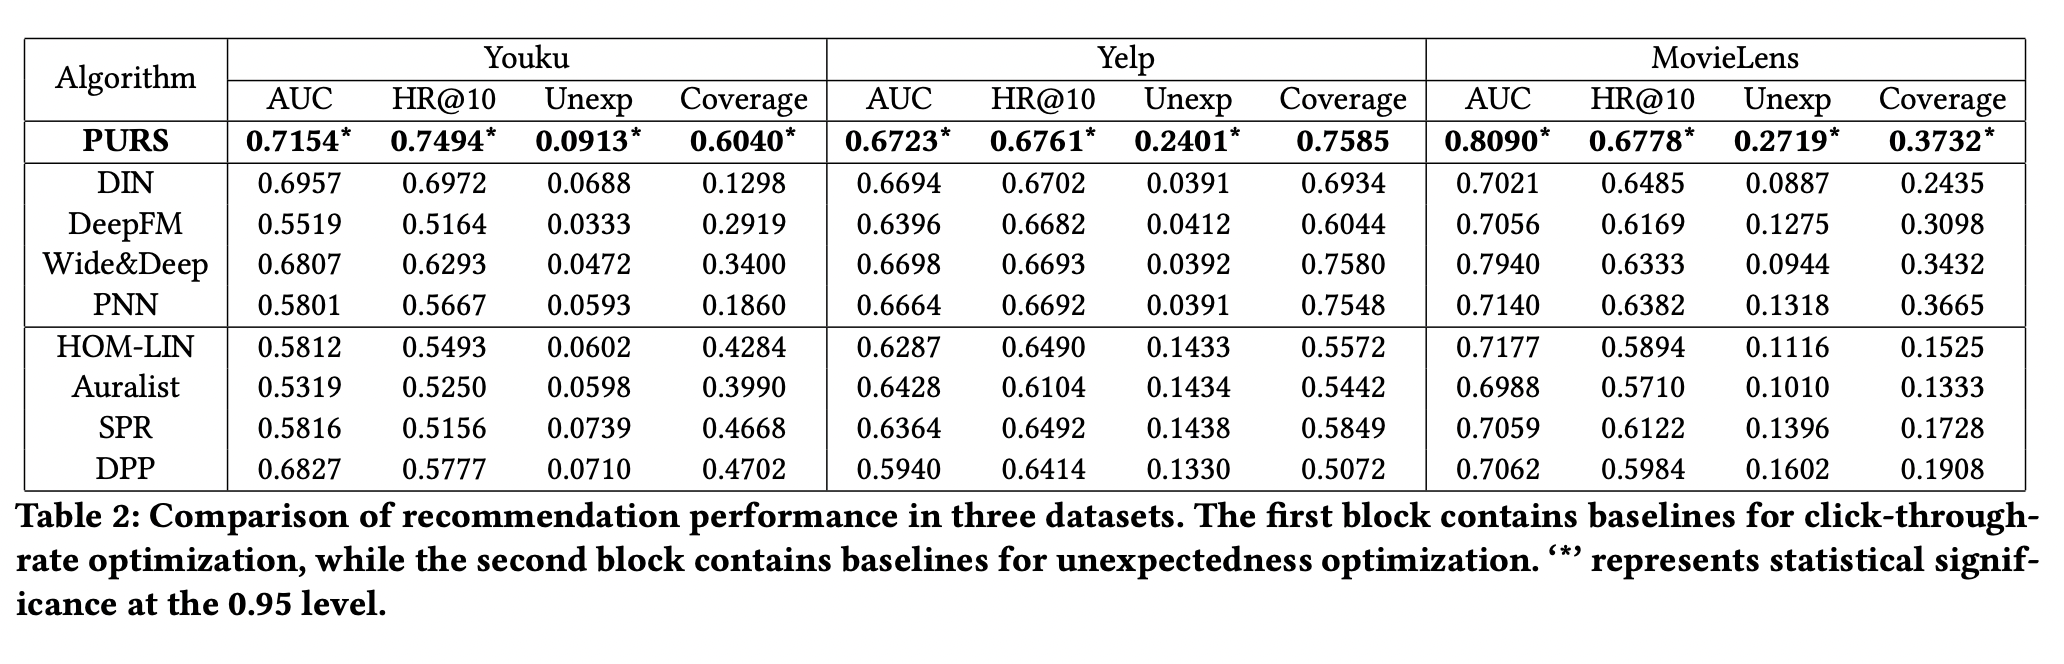
\includegraphics[width=100mm]{results.png}
    \caption{Results Comparison(from [1])
    \label{overflow}}
\end{table}
The PURS research team attributes the improvements to the following four factors: First, unexpectedness; Second, Unexpected Activation Function, which adjusts the input of unexpectedness into the utility function; Third, Personalized and Session-Based Factor, which encapsulates the user and session-level heterogeneity of perception towards unexpectedness; and finally Clustering of Behavior Sequence, which extracts the diverse user interests and constructs user expectations. Removal of any of these four components would result in a significant loss in both accuracy and unexpectedness measures. PURS is currently being deployed by Alibaba, a Chinese multinational technology company specializing in e-commerce, retail, Internet, and technology.
To conclude, the PURS model incorporates unexpectedness into the recommendation process. More precisely, user interests are represented as clusters of embedding closures in the latent space and unexpectedness is computed as the weighted distance between the new items and the interest clusters. Furthermore, the sequence modeling and the self-attention mechanism is implemented to represent personalized and session-based user perception of unexpectedness. Moreover, a novel unexpected activation function  is used in order to obtain improved unexpected recommendation performance. Finally, the CTR estimation is combined with the degree of unexpectedness to predict recommendations. The proposed PURS model surpasses baselines models both in terms of accuracy as well as novelty, successfully reducing the filter bubble effect. 

\section{A Framework for Recommending Accurate and Diverse Items  Using Bayesian Graph Convolutional Neural Networks}

The paper "A Framework for Recommending Accurate and Diverse Items  Using Bayesian Graph Convolutional Neural Networks" \footnote {Diversity in this paper means novelty} [2] introduces an alternative approach to deal with the filter bubble problem. Most existing recommender systems overlook diversity of the recommended list which leads to substandard performance. The model put forward in this paper is based on a Bayesian Graph Neural Network (BGNN). BGNNs enable the system to capture the uncertainty in the observed user-item interaction records while simultaneously bringing diversity into the recommendations.  Recently, BGNN based approaches have been used to capture the various relationships between a user and items while modeling user preferences in several personalized recommender system models. Most graph-based recommendation approaches depict the observed user-item interaction graph as a relationship between users and items resulting in sparse data. In these models, more often than not, all the unobserved user-item interactions are classified as negative samples. There are missing links that represent a given user’s possible future behavior. Also, there may be ambiguous positive interactions. To address the data sparsity issue, the researchers use Bayesian Graph Convolutional Neural Networks (BGCF) as a way to model the uncertainty in the user-item interaction graph. The BGNN incorporates a random graph generative model based on node-copying, which enables producing sample graphs similar to the observed graph. However, these graphs contain enough diversity to promote improved learning. To recap, the proposed model, BGCF, aims to tackle three big issues: 1) the sparsity issue, i.e. when user-item historical data is sparse, 2) the uncertainty issue, i.e when the data is noisy, and 3) the diversity issue, i.e. leading users to explore novel items. Currently graphs are used to model the relational data present in recommendation data sets. The user-item interaction can be represented as a bipartite graph.  The key idea in GCNs is to teach the model how to iteratively collect feature data from local graph neighborhoods using NNs.  Bayesian Personalized Ranking loss for Implicit Recommendation: The objective of the recommender system is to generate a  $total ranking>_u$ of all items for each user $u$. The graph attention network (GAT) uses self-attention operating on groups of spatially near neighbors to implicitly specify different weights for each node in a given neighborhood. The thinking behind this is that higher importance is placed on those neighbors that are more similar to the central node. GAT implemented a single-layer feedforward NN with multiple weights on sets of node feature vectors and on the transformation function to map from $\mathbb{R}^{2d}\longrightarrow\mathbb{R} $ as the attention score. Diversity (i.e. novelty) and accuracy metrics have conflicting interests: increasing one can negatively impact the other. The trade-off between diversity- in-top-$N$ and precision-in-top-$N$ is a major goal for this research. Concretely this means having a recommender system with a better accuracy/diversity trade-off leads to having more personalized recommendations without substantially sacrificing accuracy.

They show how their framework can be leveraged to infer providing a concrete formulation using the Bayesian Probabilistic Ranking training loss. As is evident in table 3.2, the testing on benchmark data sets has shown their model to be effective and to outperform state-of-the-art graph-based recommendation models. 

\begin{table}[hh!]
    \centering
    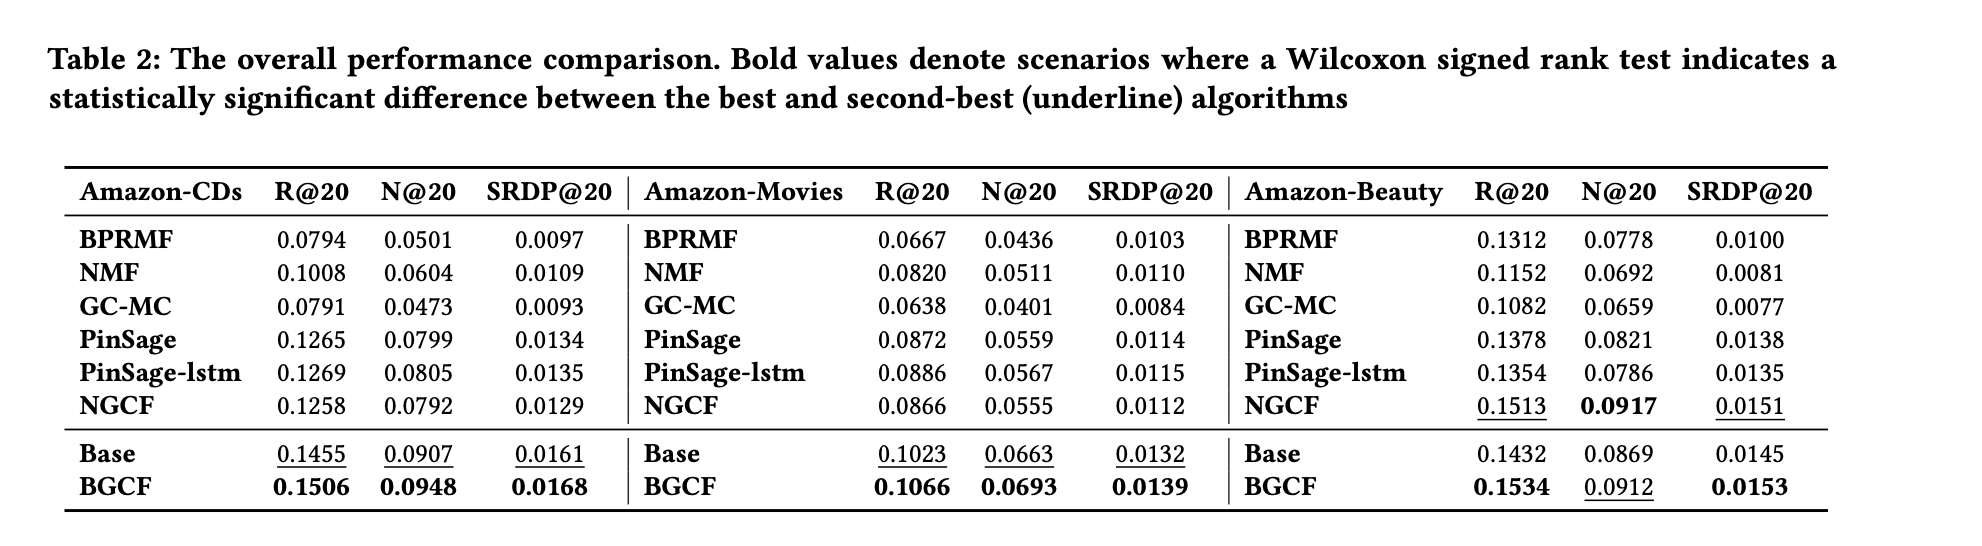
\includegraphics[width=125mm]{BGCF_results_comparison.png}
    \caption{Results Comparison (from [2])
    \label{overflow}}
\end{table}

The experiments were run on three benchmark datasets: Amazon-CDs, Amazon-Movies, and Amazon-Beauty. (Amazon-review\footnote{ http://jmcauley.ucsd.edu/data/amazon/} is a popular dataset for product recommendations: Three subsets are used here: Amazon-Movies, Beauty and CDs.) For all experiments, the recommendation accuracy of our model and baselines were assessed in terms of Recall@k and NDCG@k. Since accuracy alone does not guarantee user satisfaction, they also use serendipity@k, which factors in how surprising and relevant a recommendation is for a user. Moreover, they implement an all-scenario deep learning framework developed by Huawei, which can effectively be executed on multiple GPUs in parallel, drastically speeding up training.  Moreover, the proposed Bayesian Graph Collaborative Filtering framework incorporates diversity to the recommendations as well as alleviates the data sparsity challenges. The proposed model has the potential to be powerful for cold-start users in particular, offering a significant benefit in real-world recommender systems. 

\chapter{Multi-Armed Bandits}
According to Personalization Glossary [7] contextual bandits are defined as follows: "With the help of a relevant user data stream, contextual bandits for website optimization rely on an incoming stream of user context data, either historical or fresh, which can be used to make better algorithmic decisions in real time."
The multi-armed bandits solve the Exploration-Exploitation dilemma by striking a balance between exploration and exploitation of bandits, i.e. exploring arms which might be good and exploiting arms which are known to be good.

\section {Learning from Cross-Modal Behavior Dynamics with
Graph-Regularized Neural Contextual Bandit}

Contextual bandits is a variation of the multi-arm bandit problem. In addition to having a choice over arms, there is also a context vector. The features in the context vector include user data such as their age, the internet user behavior, etc. For each context, a choice has to be made over which arm to select. The process iterates until the best arm for each context is found[8]. In essence, the contextual multi-armed bandit problems are sequential decision problems with the goal to select the arm with the highest estimated reward in each trail, with the key idea being to learn a reward mapping function in order to infer the arm with the highest reward to pick. Many Contextual multi-armed bandit algorithms fall short of capturing complex, nonlinear inter-dependencies of user-item interactions. Additionally, these models often ignore the latent relations among users and non-recommended items, failing to properly reflect users’ preferences. Moreover, most existing approaches rely on historical data facing cold-start problems for new users with no previous user history. Learning from Cross-Modal Behavior Dynamics with Graph-Regularized Neural Contextual Bandit [4] describes an approach which focuses on resolving the aforementioned issues. The proposed Graph Regularized Cross-modal (GRC) learning model is extremely efficient in addressing and overcoming the cold-start problem. GRC is a general framework which exploits transferable data learned from user-item interactions and the external user-item features in online personalized recommendations. In particular, they exploit both positive and negative user-item interactions as well as unrecommended items through metric learning. GRC models complex user-item relationships using inherently nonlinear neural networks. Furthermore, the researchers augment GRC by combining the metric learning technique and a graph-constrained embedding module with the purpose of mapping different dimensions(temporal, social, and semantic) into the same latent space. GRC uses a multi-layer perceptron (MLP) module to grant the bandit algorithm of modelling non-linear structure of user-item relations. The great challenge is to directly derive the corresponding upper confidence bound for uncertainty estimation due to the dynamic nature in which context information is provided and the information not being strongly correlated with previous states and actions. To deal with this challenge, dropout layers are applied to learn the reward mapping function by unifying the strengths of neural network models and stochastic modeling. Also, to model the latent relations between users and items, they implement triangle inequality relation structures to capture the dependencies among positive, negative, and other unselected candidate user-item interactions. 
\begin{table}[hh!]
    \centering
    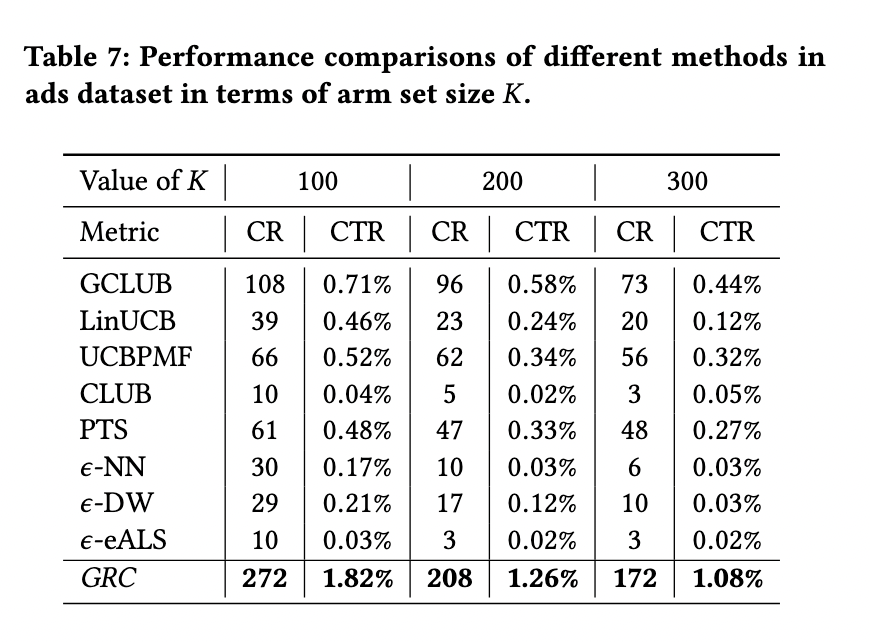
\includegraphics[width=100mm]{results_GRC.png}
    \caption{Results Comparison (from [4])
    \label{overflow}}
\end{table}
The model performance was assessed on three different datasets: 1) The LastFM Data, a dataset containing  users and artists (items) collected from a music streaming service website, 2) the Delicious Data, a social bookmarking web service data, and 3) Ads Click Stream Data, a proprietary ads click stream data from Yahoo Gemini platform. As table 4.1 shows, GRC performs better than the baselines \footnote {GCLUB, LinUCB, UCBPMF, CLUB, PTS, \textepsilon-NN, \textepsilon-DW,and \textepsilon-eALS} on all compared methods over different size of arm set. The results display the efficacy of the GRC model in capturing users’ dynamic preferences under changing settings and outperforming all baselines. The model is well-suited for capturing novel, latent, and complex user-item information.

\section{Deep Bayesian Bandits: Exploring in Online Personalized
Recommendations}
"Deep Bayesian Bandits: Exploring in  Online Personalized Recommendations" [3] offers a powerful solution to the feedback loop issue, addressing the problem of a recommender system acting greedily and favoring items already engaged by users. To combat algorithmic bias, causal inference and bandit theory and reinforcement learning (RL) are used. The model effectively employs bandit algorithms and posterior approximation algorithms for deep neural networks. Furthermore, they present a hybrid model that contains dropout units in the second-to-last layer. Confidence intervals are estimated in the UCB exploration. The proposed approach involves a trade-off between exploration and exploitation. Moreover, the exploration algorithm chooses K new items to introduce to a given user. Later, the neural network is fine-tuned using logged user actions for the predicted items. 

In addition to mitigating the filter bubble problem, Deep Bayesian Bandits is also effective against the cold-start problem. It does this by providing new information about the environment, including user preferences with the potential to result in  higher long-term rewards. More specifically, the researchers formulate a recommender as a contextual bandit problem and implement exploration techniques that require sampling from the posterior distribution -- summaries of what is known about uncertain quantities in Bayesian analysis-- of click-through-rates [4]. In their work, the researchers approximate uncertainty estimates of the predictions by implementing a bootstrapped model with multiple heads and dropout units. The context of the proposed model consists of user and item (ad) features. The model utilizes two distinct exploration algorithms: upper confidence bound(UCB) and Thompson sampling. To overcome the lack of an uncertainty estimate, they exploit neural networks, using dropout, bootstrapping, finally proposing a hybrid method that incorporates both dropout and bootstrapping. 

The model is tested following a continuous training and self-training setup. The offline model is based on Twitter data and ADS-16 dataset [26] is a publicly available dataset
that contains ratings of 300 ads shown to 120 users. The online experiments were run on a continuous data stream of 2\text{\%} of real time production traffic for 14 days. The online model was assessed on test data gathered by a random policy serving 1\text{\%} production traffic, which is representative of the distribution of the user-advertisement pairs.  Advertisement impressions are brought to users, and next, the label is published to a data stream the model’s training service is subscribing to. The model is warm-started from the previous version, and fine-tuned with newly collected data. For both the offline simulation and online simulations, the model is updated at regular intervals. The model is trained on self-generated data, forming a self-training loop. Both offline and online models were trained in a self-training loop using only data generated by that model. 

\begin{table}[hh!]
    \centering
    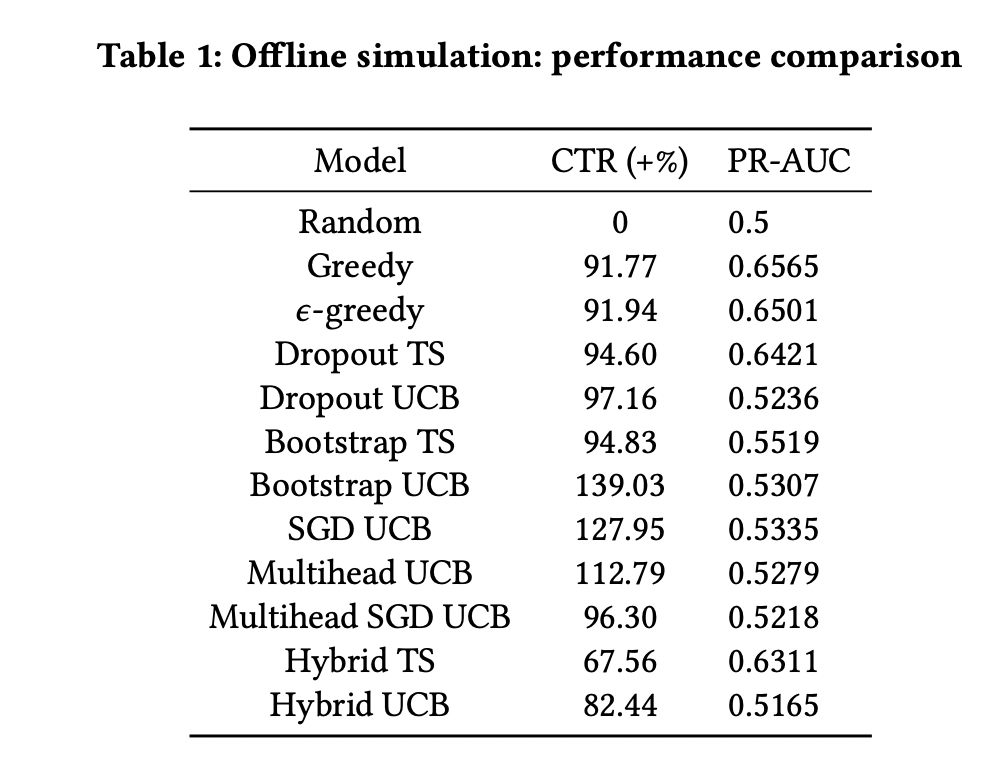
\includegraphics[width=100mm]{bandits_results.png}
    \caption{Results Comparison (from [3])
    \label{overflow}}
\end{table}

Table 4.2 shows the performance comparison in an offline experiment. For the offline simulation, a fully-connected feed-forward network. The Hybrid UCB earns more overall reward than the Hybrid TS. For example, CTR is 14.88 \text{\%}  higher for UCB than for Ts. Bootstrap UCB earns the highest rewards, but at the expense of having the highest computational cost. The performance drops with the reduction of
the computational cost of the Bootstrap UCB model by using other
variants, including the Hybrid model.
The results for the performed offline comparison
and online AB testing with large scale in-house data demonstrated high performance of the proposed model with a lower computational
cost. The model is able to address the algorithmic bias problem while simultaneously optimizing for users' long-term reward. 

\chapter{Personalized Transformer}
\section{SSE-PT Sequential Recommendation Via Personalized Transformer}

The Personalized Transformer (SSE-PT) [5] utilizes temporal data to find personalized recommendations, which is crucial for recommendation problems since user preferences in real life are dynamic in nature. Traditionally, recommender systems have primarily been based on standard collaborative filtering and ranking approaches rather than tracking sequential data. Recently, on top of powerful RNN and CNN models, attention mechanisms used in Natural Language Processing (NLP) enable the exploitation of the temporal ordering of items that users have engaged with. 
Especially the SASRec model based on the powerful NLP Transformer model has achieved impressive state-of-the-art results. Unfortunately, SASRec, is an unpersonalized model, lacking personalized user embeddings. SSE-PT is a personalized extension of the transformer model. It is sequence based, meaning that the model treats every sequence  as a given user's engagement history. The model achieves commendable results in capturing sequential, dynamic, and personalized user information. The proposed model addresses the limitations of the SASRec model outperforming it by almost 5$\%$ in terms of NDCG@10 on 5 real-world datasets. Moreover, a slightly modified SSE-PT model, which the researchers call SSE-PT++, can handle extremely long sequences, outperforming SASRec in ranking results with comparable training speed, striking a balance between performance and speed requirements. Moreover, their novel application of the Stochastic Shared Embeddings (SSE) regularization is essential to the success of personalization. Making use of user embeddings, the Personalized Transformer is able to capture a given user's recent engagement patterns. Personalization significantly improves ranking performance.
Sequential Recommendation means, "Given $n$ users with each user engaging with $m$ items in temporal order with the objective to learn a good personalized ranking of $K$ items." Sequences $s_i$ of length $T$ include indices of the most recent $T$ items that a user $i$ has interacted with in the temporal order

The application of Stochastic Shared Embeddings: Stochastic Shared Embeddings (SSE) are the most crucial regularization technique to the SSE-PT model, preventing the model from over-fitting badly after the introducing user embeddings. SSE refers to the process of 
stochastically replacing embeddings with another embedding with
a predefined probability during SGD\footnote{stochastic gradient descent}, which regularizes the embedding layers. 
\begin{table}[ht!]
    \centering
    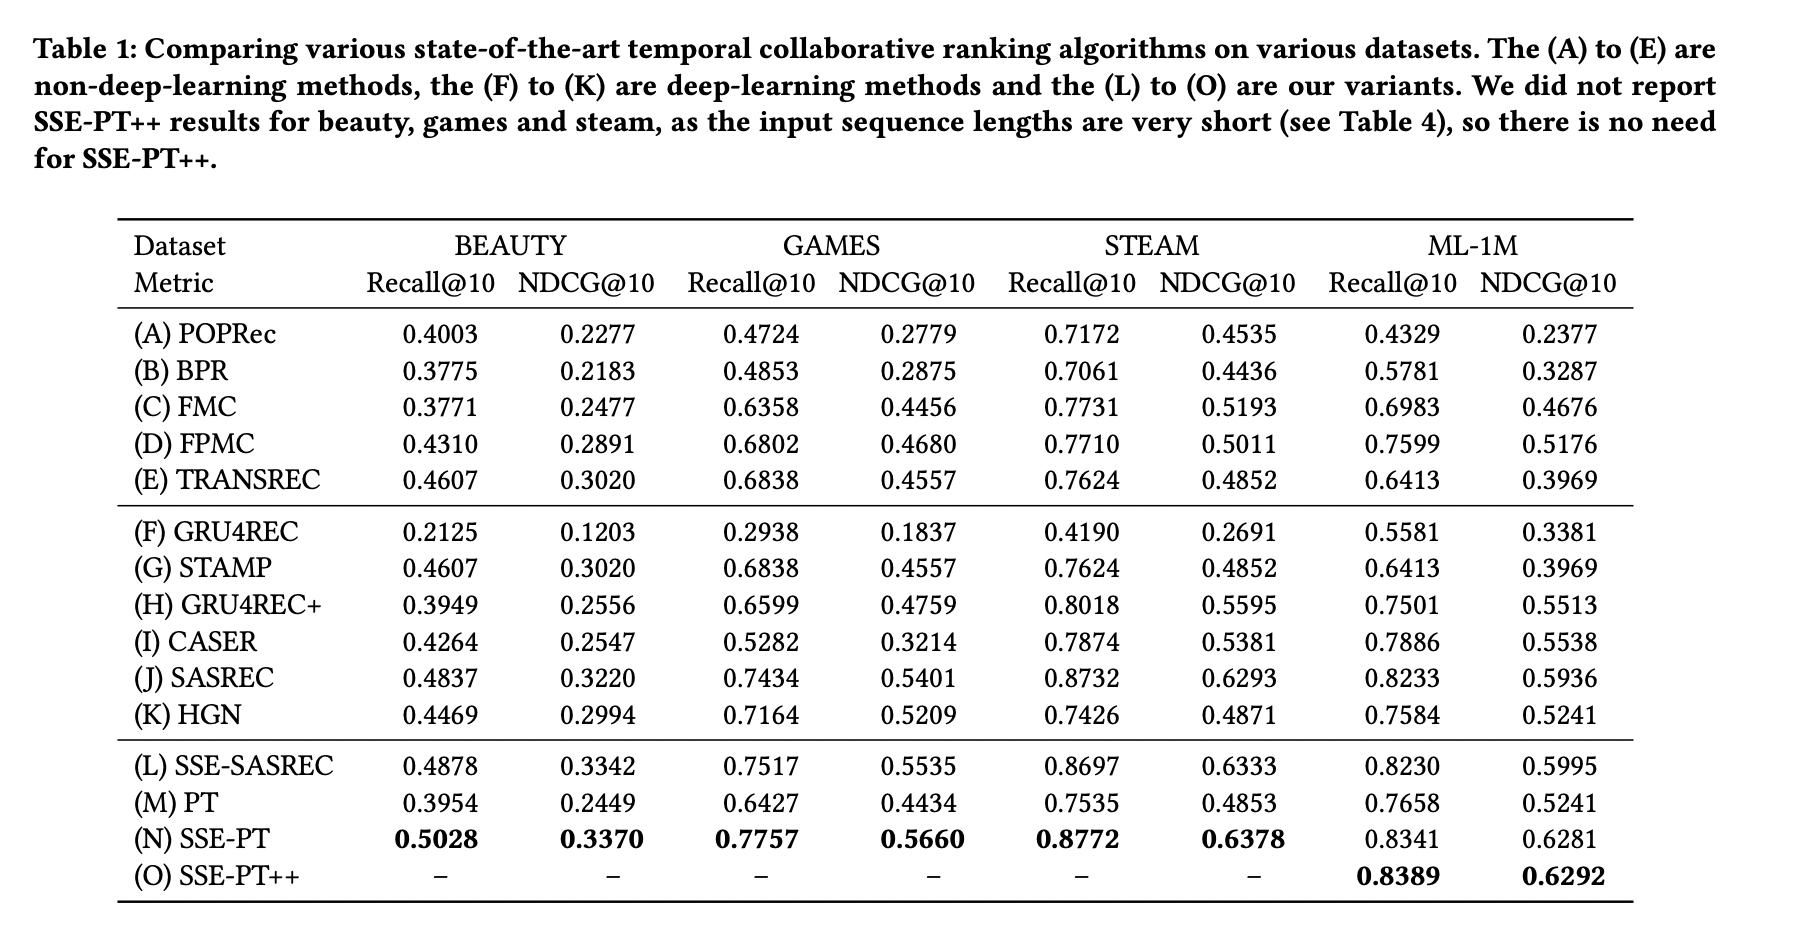
\includegraphics[width=100mm]{results_Transformer.png}
    \caption{Results Comparison (from[5])
    \label{overflow}}
\end{table}
The experiments were run on five datasets: 1) Amazon-Beauty, 2) Amazon-Games, 3) Steam -- a dataset containing reviews crawled from a large video game distribution platform, 4) Movielens 1M dataset -- a dataset containing one million user movie ratings, and 5) Movielens 10M dataset -- a dataset containing ten million user ratings cleaned by the researchers of this paper. For evaluation metrics, Normalized Discounted Cumulative Gain (NDCG) \footnote{NDCG is a popular method for measuring the quality of a set of search results} and Recall for top recommendations were used. We can see from Table 5.1 that the SSE-PT outperforms over all previous methods on the four datasets. Both SSE-PT and SSE-PT++ obtain notably better ranking performances than the baseline SASRec. SSE-PT helps mitigate the temporal collaborative ranking problem. On account of the attention mechanisms
during inference, the Personalized Transformer is also more interpretable and pays more attention to recent items in long sequences than the unpersonalized deep learning counterparts.

\chapter{ Conclusion}

All of the five models presented in this thesis have achieved remarkable results refining existing models. Effective recommender systems are vital to both businesses and individuals alike. Recommender systems help individuals in decision-making, guiding them to find interesting items in a huge pool of options. Using Recommender systems can help companies to increase their revenue and profit. The purpose of this thesis is to look into ways in which some recent, outstanding, cutting-edge recommender systems find solutions to common problems faced by current personalized recommender systems.

Modeling user interests as clusters of embedding closures while incorporating unexpectedness as the weighted distance between the novel items and the interest clusters, sequence modeling together with self-attention [1, 2, 5] as well as an adaptation of Transformer model with personalized embeddings have been shown to improve the quality of recommendations in personalized Recommender Systems. Two of the models discussed in sections  4.1. and 4.2 utilize multi-armed bandits to optimize recommendations. Furthermore, contextual bandits with deep neural networks, Bayesian Graph Neural Networks, and the use of graph-regularized cross-modal learning frameworks have proven to enhance the power of recommender systems. The five models enable efficient operations online, where new users or items arrive continually at an incredibly high rate, yielding significantly better recommendations for individual users than most existing recommender systems, providing original and potent solutions to major issues afflicting present recommender systems.
% MSc instructions
%\chapter{Johdanto}

Seuraavassa on joitain ohjeita tämän tutkielmapohjan käyttöön maisterintutkielmassa. Kirjoittamisohjeita löytyy useasta eri lähteestä. Voit esimerkiksi tutustua kandidaatintutkielman ohjeisiin. 
Ohjaajan kanssa on hyvä keskustella aikaisessa vaiheessa työn rakenteesta.

\chapter{Kuvat ja Taulukot}

\section{Kuvat}
Kuva~\ref{fig:logo} toimii esimerkkinä kuvan lisäämisestä työhön. Muista myös viitata jokaiseen kuvaan tekstissä. 

\begin{figure}[h!] % remove [h!] for automatic placement, which is probalby better for a thesis with more text on page
\centering 

\includegraphics[width=0.3\textwidth]{HY-logo-ml.png}
\caption{Helsingin yliopiston logo matemaattis-luonnontieteellisen tiedekunnan värein.\label{fig:logo}}
\end{figure}

\section{Taulukot}

Taulukossa~\ref{table:results} on esimerkki kokeellisten tulosten raportoinnista taulukkona. Muista myös viitata jokaiseen taulukkoon tekstissä.

\begin{table}[h!]
\centering
\caption{Kokeelliset tulokset.\label{table:results}}
\begin{tabular}{l||l c r} 
Koe & 1 & 2 & 3 \\ 
\hline \hline 
$A$ & 2.5 & 4.7 & -11 \\
$B$ & 8.0 & -3.7 & 12.6 \\
$A+B$ & 10.5 & 1.0 & 1.6 \\
\hline
%
\end{tabular}
\end{table}

\chapter{Viitteet}

\section{Kirjallisuusviitteet}

Kirjallisuuslähteet ylläpidetään erillisessä .bib-tiedostossa. Tässä tutkielmapohjassa käytetyt kirjallisuuslähteet, joista esimerkkejä kuvassa~\ref{bibexamples}, löytyvät tiedostosta\newline \texttt{bibliography.bib}.

\begin{figure}[h!]
    \centering
    \begin{scriptsize}
				
\begin{verbatim}

@article{einstein,
    author =       "Albert Einstein",
    title =        "{Zur Elektrodynamik bewegter K{\"o}rper}. ({German})
        [{On} the electrodynamics of moving bodies]",
    journal =      "Annalen der Physik",
    volume =       "322",
    number =       "10",
    pages =        "891--921",
    year =         "1905",
    DOI =          "http://dx.doi.org/10.1002/andp.19053221004"
}
@book{latexcompanion,
    author    = "Michel Goossens and Frank Mittelbach and Alexander Samarin",
    title     = "The \LaTeX\ Companion",
    year      = "1993",
    publisher = "Addison-Wesley",
    address   = "Reading, Massachusetts"
}
@book{knuth99,
    author    = "Donald E. Knuth",
    title     = "Digital Typography",
    year      = "1999",
    publisher = "The Center for the Study of Language and Information",
    series    = "CLSI Lecture Notes (78)"
}
\end{verbatim}
\end{scriptsize}
    \caption{Esimerkkejä kirjallisuuslähteiden kuvaamisesta .bib-tiedostossa.}
    \label{bibexamples}
\end{figure}

Viitteet kirjallisuuslähteisiin muodostetaan komennolla \texttt{\textbackslash citep\{einstein\}}, josta generoituu tekstiin valitun viittaustyylin mukaisesti muotoiltu viite \citep{einstein}, tai \texttt{\textbackslash citep\{latexcompanion,knuth99\}}, josta tekstiin puolestaan generoituu \citep{latexcompanion,knuth99}. Tekstissä viitatut kirjallisuuslähteet tulevat automaattisesti viiteluetteloon. Kirjallisuuslähteiden tietojen oikeellisuus ja yhdenmukaisuus .bib-tiedostossa vaikuttavat luonnollisesti siihen, miten tiedot tutkielmassa näyttäytyvät. Tämä on syytä huomioida, sillä esim. verkosta valmiiksi {Bib\TeX} muodossa löytyvien tietojen täydellisyyten tai samanmuotoisuuteen ei pidä sokeasti luottaa.  

Keskustele viittaustyylin valinnasta ohjaajan kanssa. Joitain vaihtoehtoja on osoitteessa:\\ 
\url{https://www.overleaf.com/learn/latex/Biblatex_bibliography_styles}.
%\url{https://www.sharelatex.com/learn/Bibtex_bibliography_styles}.

\section{Ristiviitteet}

%Liite~\ref{appendix:model} sivulla~\pageref{appendix:model} sisältää lisämateriaalia.
Taulukossa~\ref{table:results} sivulla~\pageref{table:results} on koottuna kokeelliset tulokset.

% \chapter{Pdf:n luominen tex:stä}

% Linuxissa voit ajaa komentoja \texttt{pdflatex filename.tex} ja \texttt{biber filename.tex} vuorotelleen kunnes ohjelmat eivät enää anna varoituksia. Prosessi on helppo automatisoida make-komennon avulla.
 
% \chapter{Johtopäätökset\label{chapter:conclusions}}

% Tutkielma on hyvä päättää johtopäätöksiin tutkielman löydöksistä. 

\chapter{Introduction}

The following gives some superficial instructions for using this template for a Master's thesis. For guidelines on thesis writing you can consult various sources, for example, the Bachelor thesis template.

The thesis should have an introduction chapter. Other chapters can be named according to the topic. In the end, some summary chapter is needed; see Chapter~\ref{chapter:conclusions} for an example.

\chapter{Figures and Tables}

\section{Figures}
Figure~\ref{fig:logo} gives an example how to add figures to the document. Remember always to cite the figure in the main text.

\begin{figure}[h!] 
\centering 

\includegraphics[width=0.3\textwidth]{HY-logo-ml.png}
\caption{University of Helsinki flame-logo for Faculty of Science.\label{fig:logo}}
\end{figure}

\section{Tables}

Table~\ref{table:results} gives an example how to report experimental results. Remember always to cite the table in the main text. 

\begin{table}
\centering
\caption{Experimental results.\label{table:results}}
\begin{tabular}{l||l c r} 
Experiment & 1 & 2 & 3 \\ 
\hline \hline 
$A$ & 2.5 & 4.7 & -11 \\
$B$ & 8.0 & -3.7 & 12.6 \\
$A+B$ & 10.5 & 1.0 & 1.6 \\
\hline
%
\end{tabular}
\end{table}

\chapter{Citations}

\section{Citations to literature}

References are listed in a separate .bib-file. In this case it is named \texttt{bibliography.bib} including the following content:
\begin{verbatim}
@article{einstein,
    author =       "Albert Einstein",
    title =        "{Zur Elektrodynamik bewegter K{\"o}rper}. ({German})
        [{On} the electrodynamics of moving bodies]",
    journal =      "Annalen der Physik",
    volume =       "322",
    number =       "10",
    pages =        "891--921",
    year =         "1905",
    DOI =          "http://dx.doi.org/10.1002/andp.19053221004"
}
 
@book{latexcompanion,
    author    = "Michel Goossens and Frank Mittelbach and Alexander Samarin",
    title     = "The \LaTeX\ Companion",
    year      = "1993",
    publisher = "Addison-Wesley",
    address   = "Reading, Massachusetts"
}
 
@misc{knuthwebsite,
    author    = "Donald Knuth",
    title     = "Knuth: Computers and Typesetting",
    url       = "http://www-cs-faculty.stanford.edu/%7Eknuth/abcde.html"
}
\end{verbatim}

In the last reference url field the code \verb+%7E+ will translate into \verb+~+ once clicked in the final pdf.

References are created using command \texttt{\textbackslash cite\{einstein\}}, showing as \citep{einstein}. Other examples: \citep{latexcompanion,knuthwebsite}.

Citation style can be negotiated with the supervisor. See some options in \url{https://www.sharelatex.com/learn/Bibtex_bibliography_styles}.

\section{Crossreferences}

Appendix~\ref{appendix:model} on page~\pageref{appendix:model} contains some additional material.

\chapter{From tex to pdf}

In Linux, run \texttt{pdflatex filename.tex} and \texttt{biber filename.tex} repeatedly until no more warnings are shown. This process can be automised using make-command.
Note that normally we would be using \texttt{bibtex} command instead of \texttt{biber} but because of the biblatex package \texttt{biber} should be used.
 
\chapter{Conclusions\label{chapter:conclusions}}

It is good to conclude with a summary of findings. You can also use separate chapter for discussion and future work. These details you can negotiate with your supervisor.


%%%%%%%%%%%%%%%%%%%%%%%%%%%%%%%%%%%%%%%%%%%%%%%%%%%%%%%%%
\cleardoublepage                          %fixes the position of bibliography in bookmarks
\phantomsection
\addcontentsline{toc}{chapter}{\bibname}  % This lines adds the bibliography to the ToC
\printbibliography

%%%%%%%%%%%%%%%%%%%%%%%%%%%%%%%%%%%%%%%%%%%%%%%%%%%%%%%%%
\backmatter
\begin{appendices}

%
\appendix{Template instructions}


In the HY-CS-main.tex file you will find the following STEPS 0--5. Bellow instructions what each STEP means and how to set up your thesis by following these STEPS.
\vspace{0.5cm}

\textbf{STEP 0 -- Clone the thesis template}

\begin{itemize}
\item One template for all thesis types: \url{https://www.overleaf.com/read/hzgngkgshqwh}
\end{itemize}


{\textbf{STEP 1 -- BSc or MSc thesis?}}
\begin{enumerate}
\item Select whether your are writing BSc (tkt for new, tktl for old) or MSc (csm for new, cs for old, dsm for data science) thesis.
\item Select your language: finnish, english, or swedish.
\item If you are writing MSc select your line / track.
\end{enumerate}


{\textbf{STEP 2 -- Set up your personal information}}

\begin{enumerate}
\item Write the working title of your thesis.
\item Write your name to the author field.
\item Write the names of your supervisors and examiners of the thesis.
\end{enumerate}

{\textbf{STEP 3 -- Write your abstract here}}

\begin{itemize}
\item You can also have the abstract in multiple languages with otherlanguages-environment. Bellow example how to add an english abstract to a thesis written in some other language than english: 

\begin{verbatim}
\begin{otherlanguage}{english} 
\begin{abstract}
Your abstract text goes here. 
\end{abstract} 
\end{otherlanguage}
\end{verbatim}

\end{itemize}

{\textbf{STEP 4 -- Writing your thesis}}

\begin{enumerate}
\item There are some writing instructions in [bsc/msc]\_[finnish/english]\_contents.tex files.
\item You can delete the contents of [bsc/msc]\_[finnish/english]\_contents.tex file and write your thesis inside that file.
\end{enumerate}

{\textbf{STEP 5 -- Set your bibliography style}}

\begin{itemize}
\item The default is Numbering alphabetic order, which should be used in most cases.
\end{itemize}


\appendix{Tutkielmapohjan käyttöohjeet}


HY-CS-main.tex tiedosto sisältää viisi askelta STEPS 0--5. Alla on kuvattu, mitä nämä askeleet tarkoittavat ja miten niitä seuraamalla luot itsellesi oikeanlaisen tutkielmapohjan.
\vspace{0.5cm}

\textbf{STEP 0 -- Kopioi itsellesi tutkielmapohja}

\begin{itemize}
\item Tämä sama pohja on käytössä kaikille tutkielmatyypeille:\\ \url{https://www.overleaf.com/read/hzgngkgshqwh}
\end{itemize}


{\textbf{STEP 1 -- BSc vai MSc tutkielma?}}
\begin{enumerate}
\item Valitse (tiedostossa HY-CS-main.tex) oletko tekemässä BSc (tkt uusi tutkinto, tktl vanhatutkinto) vai MSc (csm uusi tutkinto/30~op, cs vanha tutkinto/40~op)
%, dsm datatiede) 
tutkielman.
\item Valitse kieli jolla kirjoitat tutkielman: finnish, english, tai swedish.
\item Jos olet kirjoittamassa MSc tutkielmaa, valitse linja/opintosuunta.
\end{enumerate}


{\textbf{STEP 2 -- Aseta henkilökohtaiset tietosi}}

\begin{enumerate}
\item Kirjoita alustava otsikko tutkielmallesi.
\item Kirjoita oma nimesi.
\item Kirjoita ohjaajien ja tarkastajien nimet (mikäli tiedossa).
\end{enumerate}

{\textbf{STEP 3 -- Kirjoita tiivistelmä(t)}}

\begin{itemize}
\item Voit kirjoittaa tiivistelmän (koko tiivistelmäsivu) eri kielillä \texttt{otherlanguages}-ympäristön avulla. Alla esimerkki jolla kirjoitat englanninkielisen tiivistelmän muulla kuin englannin kielellä kirjoitettuun tutkielmaan:

\begin{verbatim}
\begin{otherlanguage}{english} 
\begin{abstract}
Your abstract text goes here. 
\end{abstract} 
\end{otherlanguage}
\end{verbatim}

\end{itemize}

{\textbf{STEP 4 -- Kirjoita tutkielma}}

\begin{enumerate}
\item Tutkielman kirjoittamista varten löydät ohjeita tiedostosta \newline \texttt{[bsc/msc]\_[finnish/english]\_contents.tex}.
\item Kun olet tutustunut ohjeisiin, voit poistaa tiedoston \newline \texttt{[bsc/msc]\_[finnish/english]\_contents.tex} sisällön ja kirjoittaa oman tutkielmasi kyseiseen tiedostoon.
\end{enumerate}

{\textbf{STEP 5 -- Aseta kirjallisuuslähdeluettelon tyyli}}

\begin{itemize}
\item Oletustyyli tekijä-vuosi, eli (Einstein, 1905), voit vaihtaa tyylin (tiedostossa HY-CS-main.tex) helposti kommentointia muuttamalla numeroituun, eli [1], tai aakkostyyliin, eli [Ein05].
Lisää ohjeita liittyen viittaustyylin säätämiseen {Bib}\TeX issä löytyy verkosta: \url{https://ctan.org/pkg/biblatex}

\end{itemize}


\appendix{Sample Appendix\label{appendix:model}}
usually starts on its own page, with the name and number of the appendix at the top. 
The appendices here are just models of the table of contents and the presentation. Each appendix
Each appendix is paginated separately.

In addition to complementing the main document, each appendix is also its own, independent entity.
This means that an appendix cannot be just an image or a piece of programming, but the appendix must explain its contents and meaning.

\end{appendices}
%%%%%%%%%%%%%%%%%%%%%%%%%%%%%%%%%%%%%%%%%%%%%%%%%%%%%%%%%

\end{document}
